% Documentación de la base de datos del brazo XK-JS1-1 (ETN-1000, II-2026)
% Compilar desde esta carpeta:
%   python3 generar_diccionario.py     (diccionario de datos desde el script SQL)
%   pdflatex base_datos_brazo.tex      (dos veces)
\documentclass[a4paper,11pt]{article}
% Estilo común de los manuales del gemelo digital (se incluye con \input)
\usepackage{geometry}
\geometry{letterpaper, margin=2.2cm}
\usepackage[spanish, es-nodecimaldot, mexico]{babel}
\usepackage[utf8]{inputenc}
\usepackage[T1]{fontenc}
\usepackage{lmodern}
\usepackage{amsmath,amssymb}
\usepackage[table]{xcolor}
\definecolor{naranja}{RGB}{194,98,12}
\definecolor{rojo}{RGB}{192,57,43}
\definecolor{verde}{RGB}{30,120,70}
\definecolor{azulw}{RGB}{0,103,184}
\definecolor{azulg}{RGB}{70,90,120}
\definecolor{gris}{RGB}{242,242,242}
\definecolor{grisos}{RGB}{90,90,90}
\usepackage{booktabs,longtable,array,tabularx}
\usepackage{graphicx}
\usepackage{float}
\usepackage{caption}
\captionsetup{font=small, labelfont=bf}
\usepackage{tikz}
\usetikzlibrary{positioning,arrows.meta,fit,calc,shapes.geometric,decorations.pathreplacing,backgrounds}
\usepackage{enumitem}
\setlist{itemsep=2pt}
\usepackage{listings}
\lstset{basicstyle=\ttfamily\small, frame=single, backgroundcolor=\color{gris}, breaklines=true,
  columns=fullflexible, keepspaces=true, extendedchars=true, upquote=true,
  literate={á}{{\'a}}1 {é}{{\'e}}1 {í}{{\'i}}1 {ó}{{\'o}}1 {ú}{{\'u}}1 {ñ}{{\~n}}1 {Á}{{\'A}}1 {É}{{\'E}}1
           {Í}{{\'I}}1 {Ó}{{\'O}}1 {Ú}{{\'U}}1 {Ñ}{{\~N}}1 {ü}{{\"u}}1 {¿}{{?`}}1 {¡}{{!`}}1 {…}{{...}}3
           {θ}{{$\theta$}}1 {·}{{$\cdot$}}1 {«}{{\guillemotleft}}1 {»}{{\guillemotright}}1 {°}{{$^\circ$}}1}
\usepackage{hyperref}
\hypersetup{colorlinks=true, linkcolor=naranja, urlcolor=naranja}
\usepackage{fancyhdr}
\pagestyle{fancy}
\fancyhf{}
\cfoot{\small \thepage}
\newcommand{\codigo}[1]{\texttt{#1}}
\newcommand{\archivo}[1]{\textbf{\texttt{#1}}}
\newcommand{\aviso}[1]{\par\smallskip\noindent\colorbox{rojo!10}{\parbox{\dimexpr\linewidth-2\fboxsep}{\textbf{\color{rojo}Atención.} #1}}\par\smallskip}
\newcommand{\nota}[1]{\par\smallskip\noindent\colorbox{gris}{\parbox{\dimexpr\linewidth-2\fboxsep}{#1}}\par\smallskip}
\tikzset{
  marca/.style={circle, fill=naranja, text=white, font=\bfseries\footnotesize, inner sep=1.4pt, minimum size=4.6mm, draw=white, line width=0.8pt},
  caja/.style={draw, rounded corners=2pt, fill=gris, align=center, font=\small, minimum height=10mm, inner sep=4pt},
  cajab/.style={caja, fill=white},
  cajan/.style={caja, fill=naranja!14, draw=naranja!70!black},
  paso/.style={draw, rounded corners=2pt, fill=white, align=left, font=\small, text width=3.4cm, minimum height=15mm, inner sep=5pt},
  num/.style={circle, fill=naranja, text=white, font=\bfseries\small, inner sep=1.5pt, minimum size=6mm},
  flecha/.style={-{Stealth[length=2.2mm]}, thick},
  dflecha/.style={{Stealth[length=2.2mm]}-{Stealth[length=2.2mm]}, thick},
  etiq/.style={font=\scriptsize, align=center},
}
\DeclareRobustCommand{\num}[1]{\tikz[baseline=-0.7ex]\node[marca]{#1};}
% \captura{ancho}{archivo}{marcas en coordenadas 0-1 desde la esquina inferior izquierda}
\newcommand{\captura}[3]{%
  \begin{tikzpicture}
  \node[anchor=south west, inner sep=0, draw=black!25] (img) {\includegraphics[width=#1]{#2}};
  \begin{scope}[x={(img.south east)}, y={(img.north west)}]
  #3
  \end{scope}
  \end{tikzpicture}}
% ventana dibujada (consolas y diálogos): \ventana{ancho}{alto}{título}{contenido}
\newcommand{\ventana}[4]{%
\begin{tikzpicture}
\node[draw=black!50, fill=white, minimum width=#1, minimum height=#2, anchor=north west, inner sep=0] (v) at (0,0) {};
\fill[black!8] (v.north west) rectangle ($(v.north east)+(0,-6mm)$);
\node[anchor=west, font=\scriptsize] at ($(v.north west)+(2mm,-3mm)$) {#3};
\node[anchor=east, font=\scriptsize] at ($(v.north east)+(-2mm,-3mm)$) {--\quad$\square$\quad$\times$};
\node[anchor=north west, inner sep=3mm, text width=#1-6mm, font=\scriptsize\ttfamily, align=left] at ($(v.north west)+(0,-6mm)$) {#4};
\end{tikzpicture}}

% Macros del manual técnico: ladder, estados, código y rutas de imágenes
\usetikzlibrary{shapes.multipart}
\graphicspath{{../img/}{../../../../../../../global/fotos-planta/}{../../../modelo-3d/informe/figuras/}{../../../modelo-3d/levantamiento/}{../../../../../database/modelo/}{../../../../../documentacion/manuales_inversa/}{../../../../../documentacion/planos_isa/electrico/}{../../../../../database/interfaz/}}

\lstdefinestyle{py}{language=Python, keywordstyle=\color{azulg}\bfseries, commentstyle=\color{grisos}\itshape,
  stringstyle=\color{verde}, basicstyle=\ttfamily\scriptsize, numbers=left, numberstyle=\tiny\color{grisos}}
\lstdefinestyle{js}{language=Java, morekeywords={const,let,function,async,await,return,for,of,if,else}, keywordstyle=\color{azulg}\bfseries,
  commentstyle=\color{grisos}\itshape, stringstyle=\color{verde}, basicstyle=\ttfamily\scriptsize, numbers=left, numberstyle=\tiny\color{grisos}}
\lstdefinestyle{awl}{basicstyle=\ttfamily\tiny, commentstyle=\color{grisos}\itshape, morecomment=[l]{//},
  keywordstyle=\color{azulg}\bfseries, morekeywords={LD,LDN,A,AN,O,ON,EU,ED,S,R,MOVB,MOVW,MOVD,PLS,TON,CALL,CRET,LPS,LRD,LPP,ALD,OLD,FILL,LDW,LDB,LDD,AW,AD,AB,OW,OD},
  numbers=left, numberstyle=\tiny\color{grisos}, frame=single, backgroundcolor=\color{gris}}
\lstdefinestyle{sql}{language=SQL, keywordstyle=\color{azulg}\bfseries, commentstyle=\color{grisos}\itshape,
  stringstyle=\color{verde}, basicstyle=\ttfamily\tiny, numbers=left, numberstyle=\tiny\color{grisos},
  morekeywords={REFERENCES,SERIAL,SMALLSERIAL,BIGSERIAL,TIMESTAMPTZ,BOOLEAN,INET,RETURNS,TRIGGER,LANGUAGE,DECLARE,RAISE,EXCEPTION,VIEW,INDEX}}

\tikzset{
  ld/.style={line width=0.7pt},
  pics/na/.style={code={\fill[white](-0.12,-0.26) rectangle (0.12,0.26);
     \draw[thick](-0.1,-0.24)--(-0.1,0.24)(0.1,-0.24)--(0.1,0.24);
     \node[font=\scriptsize\ttfamily, above] at (0,0.22){#1};}},
  pics/nc/.style={code={\fill[white](-0.12,-0.26) rectangle (0.12,0.26);
     \draw[thick](-0.1,-0.24)--(-0.1,0.24)(0.1,-0.24)--(0.1,0.24);\draw(-0.17,-0.24)--(0.17,0.24);
     \node[font=\scriptsize\ttfamily, above] at (0,0.22){#1};}},
  pics/pf/.style={code={\fill[white](-0.12,-0.26) rectangle (0.12,0.26);
     \draw[thick](-0.1,-0.24)--(-0.1,0.24)(0.1,-0.24)--(0.1,0.24);
     \node[font=\tiny\bfseries] at (0,0){P};}},
  pics/cmp/.style n args={3}{code={\fill[white](-0.12,-0.26) rectangle (0.12,0.26);
     \draw[thick](-0.1,-0.24)--(-0.1,0.24)(0.1,-0.24)--(0.1,0.24);
     \node[font=\tiny\ttfamily] at (0,0){#2};
     \node[font=\scriptsize\ttfamily, above] at (0,0.22){#1};
     \node[font=\scriptsize\ttfamily, below] at (0,-0.22){#3};}},
  pics/bob/.style n args={3}{code={\fill[white](-0.2,-0.26) rectangle (0.2,0.26);
     \draw[thick](-0.05,0.24) arc (110:250:0.255);\draw[thick](0.05,0.24) arc (70:-70:0.255);
     \node[font=\tiny\bfseries] at (0,0){#2};
     \node[font=\scriptsize\ttfamily, above] at (0,0.22){#1};
     \node[font=\scriptsize\ttfamily, below] at (0,-0.22){#3};}},
  fb/.style={draw, fill=white, font=\scriptsize\ttfamily, align=left, inner sep=3pt, anchor=west},
  barra/.style={line width=2pt},
  estado/.style={draw, rounded corners=3pt, fill=white, align=center, font=\scriptsize, minimum width=22mm, minimum height=10mm, inner sep=3pt},
  estadon/.style={estado, fill=naranja!14, draw=naranja!70!black},
  trans/.style={font=\scriptsize, align=center, fill=white, inner sep=1pt},
  lugar/.style={circle, draw, thick, minimum size=7mm, fill=white},
  transicion/.style={rectangle, fill=black, minimum width=1.6mm, minimum height=7mm, inner sep=0},
  tabla/.style={rectangle split, rectangle split parts=2, draw, fill=white, font=\tiny\ttfamily, align=left, inner sep=2pt, rounded corners=1pt, text width=33mm},
}
\newcommand{\pendiente}[1]{\par\smallskip\noindent\colorbox{naranja!12}{\parbox{\dimexpr\linewidth-2\fboxsep}{\textbf{\color{naranja!80!black}Pendiente.} #1}}\par\smallskip}
\newcommand{\cumple}{\textcolor{verde}{\textbf{cumplido}}}
\newcommand{\parcial}{\textcolor{naranja}{\textbf{parcial}}}
\newcommand{\falta}{\textcolor{rojo}{\textbf{pendiente}}}

\graphicspath{{../../../../database/modelo/}{../../../../database/mockups/}{../../../../database/interfaz/}}
\usepackage{pdflscape}
\usepackage{tocloft}
\setlength{\cftsecnumwidth}{2.2em}
\setlength{\cftsubsecnumwidth}{2.8em}
\setlength{\cftbeforesecskip}{3pt}
\usetikzlibrary{shapes.geometric}
\lhead{\small Brazo XK-JS1-1 · Base de datos}
\rhead{\small ETN-1000 · II/2026}
\setlength{\headheight}{14pt}
\lstset{showstringspaces=false}

\tikzset{
  ent/.style={draw, thick, fill=white, minimum width=24mm, minimum height=8mm, align=center, font=\scriptsize\bfseries},
  entd/.style={ent, double, double distance=1.2pt},
  relc/.style={diamond, draw, fill=naranja!12, aspect=2.1, inner sep=0.6pt, font=\tiny, align=center},
  atr/.style={ellipse, draw, fill=white, font=\tiny, inner sep=1pt},
  lin/.style={thick, black!70},
  cd/.style={font=\tiny\bfseries, fill=white, inner sep=0.8pt},
  tl/.style={rectangle split, rectangle split parts=2, draw, thick, fill=white, font=\tiny\ttfamily, align=left,
             inner sep=2.2pt, text width=#1, rectangle split part fill={naranja!18, white}},
  tl/.default=41mm,
  proc/.style={circle, draw, thick, fill=naranja!10, minimum size=19mm, align=center, font=\scriptsize},
  extd/.style={draw, thick, fill=gris, minimum height=9mm, align=center, font=\scriptsize, inner sep=3pt},
  alm/.style={draw=none, minimum height=6mm, align=left, font=\scriptsize, inner sep=2pt, path picture={
     \draw[thick] (path picture bounding box.north west) -- (path picture bounding box.north east)
                  (path picture bounding box.south west) -- (path picture bounding box.south east)
                  ([xshift=7mm]path picture bounding box.north west) -- ([xshift=7mm]path picture bounding box.south west);}},
}
% columna PK / FK en el modelo lógico
\newcommand{\pk}[1]{\underline{\textbf{#1}}}
\newcommand{\fk}[1]{\textit{#1}}

\begin{document}

\begin{titlepage}
\centering
\vspace*{1.5cm}
{\large Universidad Mayor de San Andrés · Facultad de Ingeniería · Ingeniería Electrónica\par}
\vspace{1.0cm}
{\color{naranja!80!black}\rule{\linewidth}{1.5pt}\par}
\vspace{0.4cm}
{\Huge\bfseries Base de datos del brazo XK-JS1-1\par}
\vspace{0.3cm}
{\LARGE Modelo, normalización, scripts y diagramas\par}
\vspace{0.3cm}
{\color{naranja!80!black}\rule{\linewidth}{1.5pt}\par}
\vspace{1cm}
{\large ETN-1000 Bases de Datos · en conjunto con ETN-902 y ETN-1034\par}
\vspace{0.3cm}
{\large Laboratorio integrado · gestión II/2026\par}
\vspace{1.2cm}
\begin{tikzpicture}[node distance=5mm and 14mm]
\node[cajab] (p) {Planta\\\scriptsize PLC S7-200};
\node[cajab, right=of p] (a) {App del\\gemelo digital};
\node[cajan, right=of a] (b) {PostgreSQL\\\scriptsize\codigo{brazo4gdl}};
\node[cajab, right=of b] (d) {Dashboard\\\scriptsize KPIs e historial};
\draw[flecha] (p) -- node[above, etiq]{PPI} (a);
\draw[flecha] (a) -- node[above, etiq]{SQL} (b);
\draw[flecha] (b) -- node[above, etiq]{consultas} (d);
\end{tikzpicture}
\vfill
{\large Docente: Ing. Jorge Antonio Nava Amador\par}
\vspace{0.3cm}
{Equipo de control: Gabriel Andres Gomez Calla · Jose Lenin Mamani Choque · Miguel Alejandro Lima Huarachi · Román Abner Machicado Arequipa\par}
\vspace{0.5cm}
{\small La Paz, noviembre de 2026\par}
\end{titlepage}

{\setlength{\parskip}{0pt}\tableofcontents}
\newpage

% =====================================================================
\section{Qué piden las guías y dónde se cumple}\label{sec:objetivos}

Las tres guías del laboratorio integrado reparten el trabajo de la base de datos a lo largo del Ciclo de Vida del Desarrollo de Sistemas (SDLC). La tabla resume cada requisito de ETN-1000, la sección de este documento que lo responde y su estado.

\begin{longtable}{>{\raggedright}p{0.9cm} >{\raggedright}p{6.2cm} >{\raggedright}p{5.0cm} >{\raggedright\arraybackslash}p{2.5cm}}
\toprule
\textbf{Guía} & \textbf{Requisito} & \textbf{Dónde} & \textbf{Estado}\\
\midrule
\endhead
1 & Arquitectura de un RDBMS frente a archivos de texto & Sección \ref{sec:rdbms} & \cumple\\
1 & Levantamiento de las necesidades de datos de la planta & Sección \ref{sec:requerimientos} & \cumple\\
1 & Modelo E-R y normalización (1FN, 2FN, 3FN) & Secciones \ref{sec:er}, \ref{sec:logico} y \ref{sec:normalizacion} & \cumple\\
1 & SQL puro (DDL y DML): tablas, llaves primarias y foráneas, índices para búsquedas por marca de tiempo & Sección \ref{sec:script}, \archivo{scripts/brazo\_4gdl.sql} & \cumple\\
1 y 5 & Triggers PL/pgSQL que impidan datos nulos o fuera de rango, registren la alerta y cambien el estado de la planta & Sección \ref{sec:reglas}, \archivo{scripts/prueba\_reglas.sql} & \cumple\ (probado en PostgreSQL 16.2)\\
1 & Instalar PostgreSQL en la PC del laboratorio & Sección \ref{sec:instalar} & \parcial\ (probado en la PC de desarrollo)\\
1 & Middleware que lea la planta e inserte en PostgreSQL & Sección \ref{sec:flujo} (lectura PPI hecha; inserción propuesta) & \parcial\\
1 & KPIs en el dashboard web & Sección \ref{sec:consultas}, \archivo{scripts/consultas\_kpi.sql} & \parcial\ (consultas listas)\\
2 & Mockups de la interfaz local y del dashboard & carpeta \archivo{mockups/} & \cumple\\
2 & Justificar el flujo SDLC que conecta los planos técnicos con los requerimientos de la base & Secciones \ref{sec:sdlc} y \ref{sec:mockups} & \cumple\\
3 & Modelo E-R formal y modelo lógico desde los requerimientos y los mockups & Secciones \ref{sec:er} y \ref{sec:logico} & \cumple\\
3 & Telemetría histórica de las variables PV, MV y DV & Secciones \ref{sec:requerimientos} y \ref{sec:tags} & \parcial\ (DV sin sensor)\\
3 & Estados de las alarmas críticas & tablas \codigo{alarma} y \codigo{evento\_alarma} & \cumple\\
3 & Registro de inicio de sesión de los operadores (logs) & tablas \codigo{usuario}, \codigo{rol}, \codigo{sesion} & \cumple\\
3 & Normalización rigurosa, paso a paso & Sección \ref{sec:normalizacion} & \cumple\\
3 & El E-R refleja los tags ISA-5.1 de los lazos de control & Sección \ref{sec:tags} & \cumple\\
3 & Diagrama E-R y lógico con PK, FK, tipos y cardinalidades (1:N, M:N) & Figuras \ref{fig:er}, \ref{fig:log1}--\ref{fig:log3} y diccionario (sección \ref{sec:diccionario}) & \cumple\\
3 & Herramienta CASE (pgModeler o MySQL Workbench) & Sección \ref{sec:case} & \parcial\\
3 & Repositorio con código de base de datos, middleware y CAD & Sección \ref{sec:repo} & \cumple\\
\bottomrule
\end{longtable}

% =====================================================================
\section{Del plano a la base de datos: el flujo SDLC}\label{sec:sdlc}

La base de datos no se diseñó aislada: cada tabla viene de algo que el equipo de control levantó antes en la planta. El orden fue el de la figura \ref{fig:sdlc}.

\begin{figure}[H]
\centering
\begin{tikzpicture}[node distance=4mm and 6mm, every node/.style={font=\scriptsize}]
\node[paso] (l1) {\textbf{Lab 1 · Auditoría}\\variables PV, MV, DV\\señales del PLC\\informe 1};
\node[paso, right=of l1] (l2) {\textbf{Lab 2 · Planos v2.0}\\P\&ID con tags ISA\\esquema eléctrico\\mockups de la HMI};
\node[paso, right=of l2] (l3) {\textbf{Lab 3 · Modelo}\\E-R conceptual\\modelo lógico 3FN\\repositorio Git};
\node[paso, right=of l3] (f2) {\textbf{Fase 2 · Script}\\DDL, DML\\triggers, índices\\vistas};
\node[paso, below=8mm of f2] (f3) {\textbf{Fase 3 · Integración}\\middleware Python\\inserción por PPI\\dashboard};
\node[paso, left=of f3] (k) {\textbf{Kaizen}\\revisión con los datos reales: nueva versión};
\draw[flecha] (l1) -- (l2); \draw[flecha] (l2) -- (l3); \draw[flecha] (l3) -- (f2); \draw[flecha] (f2) -- (f3);
\draw[flecha] (f3) -- (k); \draw[flecha, dashed] (k) -| (l2);
\end{tikzpicture}
\caption{Flujo SDLC de las guías 1 a 3: los planos y los mockups son los requerimientos de la base de datos.}\label{fig:sdlc}
\end{figure}

\begin{center}\small
\begin{tabularx}{\linewidth}{>{\raggedright}p{5.2cm} >{\raggedright\arraybackslash}X}
\toprule
\textbf{Artefacto previo} & \textbf{Qué aportó a la base}\\
\midrule
Tabla de E/S del PLC (manual técnico, cap.~2) & las 22 filas de \codigo{punto\_io}: dirección, tipo de señal y descripción\\
P\&ID v2.0 (\codigo{planos/pid/brazo\_pid\_v2.pdf}) & los tags ISA (\codigo{tag\_isa}) y el número de lazo de cada eje (\codigo{eje.lazo\_isa})\\
Esquema eléctrico v2.0 (\codigo{planos/electrico/}) & qué salida mueve qué eje (K1, K2, PTO compartido) y la columna \codigo{punto\_io.eje\_id}\\
Clasificación PV, MV, DV (Lab 1) & \codigo{variable.clase} y los rangos que usa el trigger\\
Calibración de los ejes (cap.~5 del manual) & \codigo{eje.pulsos\_unidad} y los rangos de recorrido\\
Mockups del Lab 2 & las consultas del dashboard (sección \ref{sec:mockups})\\
App del gemelo digital (registro, \codigo{usuarios.json}) & órdenes, rechazos, sesiones y roles\\
Modelo E-R preliminar del equipo & punto de partida de la normalización (sección \ref{sec:normalizacion})\\
\bottomrule
\end{tabularx}
\end{center}

% =====================================================================
\section{Por qué un RDBMS y no archivos de texto}\label{sec:rdbms}

Hoy la app del gemelo digital guarda lo que pasa en dos archivos: \codigo{registro\_gemelo.log} (texto, una línea por evento) y \codigo{usuarios.json}. Sirven para depurar, pero no para analizar:

\begin{center}\small
\begin{tabularx}{\linewidth}{>{\raggedright}p{3.4cm} >{\raggedright}X >{\raggedright\arraybackslash}X}
\toprule
\textbf{Aspecto} & \textbf{Archivo de texto (hoy)} & \textbf{PostgreSQL (propuesto)}\\
\midrule
Consultas & leer todo el archivo y buscar texto & SQL con filtros, uniones y agregados\\
Búsquedas por tiempo & recorrido lineal & índice B-tree sobre \codigo{(variable\_id, instante)}\\
Integridad & cualquier línea es válida & tipos, NOT NULL, CHECK, claves foráneas, triggers\\
Concurrencia & riesgo si escriben dos hilos & transacciones ACID\\
Seguridad & permisos del archivo & roles y permisos por tabla\\
Acceso remoto & copiar el archivo & conexión TCP (puerto 5432) desde el dashboard\\
Crecimiento & un archivo cada vez más grande & tablas particionables por fecha\\
\bottomrule
\end{tabularx}
\end{center}

% =====================================================================
\section{Requerimientos de datos}\label{sec:requerimientos}

\subsection{Qué debe guardar la base}
Del levantamiento del Lab 1 y de la guía 3, la base debe guardar seis grupos de datos:
\begin{enumerate}
\item \textbf{Catálogo de la planta}: sistema, ejes, señales del PLC, variables con su unidad y rango, programas del PLC.
\item \textbf{Telemetría} de las variables continuas (PV, MV) con marca de tiempo.
\item \textbf{Cambios de estado} de las señales digitales: finales de carrera, sensor inductivo, relés, garra.
\item \textbf{Operación}: ciclos (cuándo y en qué modo se usó la planta) y órdenes de control (quién, qué, a qué destino, aceptada o no).
\item \textbf{Alarmas}: catálogo y eventos de activación y normalización.
\item \textbf{Seguridad}: usuarios, roles y registro de ingresos.
\end{enumerate}

\subsection{Variables del proceso}
\begin{center}\small
\begin{tabularx}{\linewidth}{c >{\ttfamily}p{1.6cm} >{\raggedright}p{4.2cm} c >{\raggedright\arraybackslash}X}
\toprule
\textbf{Clase} & \textrm{\textbf{Tag}} & \textbf{Variable} & \textbf{Unidad} & \textbf{Cómo se obtiene}\\
\midrule
PV & ZI-101 & posición de la base $\theta$ & ° & pulsos contados por el PLC / 190,3 pulsos/°\\
PV & ZI-102 & posición del carro X & mm & pulsos / 200 pulsos/mm, 0 a 170 mm\\
PV & ZI-103 & posición del carro Y & mm & pulsos / 200 pulsos/mm, 0 a 170 mm\\
MV & SY-101 & frecuencia del tren de la base & Hz & PTO0 (Q0.0)\\
MV & SY-100 & frecuencia del tren X/Y & Hz & PTO1 (Q0.1), compartido por K1 y K2\\
DV & -- & carga en la garra, fricción, pérdida de pasos & -- & sin sensor: no se puede medir (ver nota)\\
\bottomrule
\end{tabularx}
\end{center}

\nota{\textbf{Sobre las DV.} La base ya acepta la clase \codigo{DV} en \codigo{variable.clase}, pero la planta no tiene ningún sensor que mida una perturbación: el brazo trabaja en lazo abierto, sin encoders. Por eso no se cargó ninguna fila DV con un rango inventado. Cuando se agregue un sensor (por ejemplo, una celda de carga en la garra o un encoder que permita medir la pérdida de pasos), basta con insertar la variable con su tag, unidad y rango: el resto del modelo no cambia.}

\subsection{Alarmas}
Las nueve alarmas del catálogo salen de los mensajes de error que ya produce la app, de los avisos del programa del PLC y del trigger de seguridad:
\begin{center}\small
\begin{tabular}{>{\ttfamily}l c l}
\toprule
\textrm{\textbf{Código}} & \textbf{Severidad} & \textbf{Significado}\\
\midrule
comunicacion & 2 & se perdió la comunicación PPI\\
watchdog & 3 & el PLC detuvo un movimiento porque la PC dejó de dar señales de vida\\
paro & 2 & paro por pulsador, selector u orden de la PC\\
fuera\_de\_rango & 1 & destino fuera del recorrido\\
sin\_homing & 1 & orden de movimiento sin referencia\\
ocupado & 1 & orden con un movimiento en curso\\
falla\_homing & 3 & homing sin sensor o con tiempo excedido\\
posicion\_incierta & 2 & tramo interrumpido: hace falta un nuevo homing\\
limite\_variable & 3 & una variable medida salió de su rango seguro (la registra el trigger)\\
\bottomrule
\end{tabular}
\end{center}

% =====================================================================
\section{Modelo conceptual entidad-relación}\label{sec:er}

El modelo conceptual (figura \ref{fig:er}) usa la notación de Chen: los rectángulos son entidades, los rombos son relaciones y los números en los extremos son la cardinalidad máxima. Para que el diagrama se lea, los atributos van en el modelo lógico (sección \ref{sec:logico}) y en el diccionario (sección \ref{sec:diccionario}). Solo se dibuja el atributo \emph{valor} de la relación \emph{destino}, porque es el único que pertenece a una relación y no a una entidad.

\begin{landscape}
\begin{figure}[p]
\centering
\begin{tikzpicture}[x=1cm, y=1cm]
% --- seguridad (izquierda)
\node[ent] (rol) at (1.5,14) {ROL};
\node[relc] (asigna) at (1.5,12.25) {asigna};
\node[ent] (usu) at (1.5,10.5) {USUARIO};
\node[relc] (abre) at (1.5,8.75) {abre};
\node[ent] (ses) at (1.5,7) {SESION};
\draw[lin] (rol) -- node[cd, pos=0.25]{1} (asigna) -- node[cd, pos=0.75]{N} (usu);
\draw[lin] (usu) -- node[cd, pos=0.25]{1} (abre) -- node[cd, pos=0.75]{N} (ses);
% --- órdenes
\node[ent] (ord) at (7,10.5) {ORDEN};
\node[relc] (emite) at (4.25,10.5) {emite};
\draw[lin] (usu) -- node[cd, pos=0.3]{1} (emite) -- node[cd, pos=0.7]{N} (ord);
\node[relc] (dest) at (10.5,10.5) {destino};
\node[atr] (val) at (10.5,12.1) {valor};
\draw[lin] (dest) -- (val);
\node[ent] (eje) at (14.5,10.5) {EJE};
\draw[lin] (ord) -- node[cd, pos=0.3]{M} (dest) -- node[cd, pos=0.7]{N} (eje);
% --- planta
\node[ent] (sis) at (14.5,14) {SISTEMA};
\node[relc] (tiene) at (14.5,12.25) {tiene};
\draw[lin] (sis) -- node[cd, pos=0.25]{1} (tiene) -- node[cd, pos=0.75]{N} (eje);
\node[ent] (pio) at (20.5,10.5) {PUNTO\_IO};
\node[relc] (agrupa) at (17.5,10.5) {agrupa};
\draw[lin] (eje) -- node[cd, pos=0.3]{1} (agrupa) -- node[cd, pos=0.7]{N} (pio);
\node[relc] (posee) at (20.5,12.25) {posee};
\draw[lin] (sis) -| node[cd, pos=0.12]{1} (posee); \draw[lin] (posee) -- node[cd, pos=0.6]{N} (pio);
\node[ent] (var) at (14.5,7) {VARIABLE};
\node[relc] (mide) at (14.5,8.75) {mide};
\draw[lin] (eje) -- node[cd, pos=0.25]{1} (mide) -- node[cd, pos=0.75]{N} (var);
\node[ent] (est) at (20.5,7) {ESTADO\_IO};
\node[relc] (cambia) at (20.5,8.75) {cambia};
\draw[lin] (pio) -- node[cd, pos=0.25]{1} (cambia) -- node[cd, pos=0.75]{N} (est);
\node[ent] (mue) at (14.5,3.5) {MUESTRA};
\node[relc] (medida) at (14.5,5.25) {se mide en};
\draw[lin] (var) -- node[cd, pos=0.25]{1} (medida) -- node[cd, pos=0.75]{N} (mue);
% --- operación
\node[ent, minimum height=12mm] (cic) at (7,5) {CICLO\_OPERACION};
\node[relc] (cont) at (7,7.75) {contiene};
\draw[lin] (cic) -- node[cd, pos=0.25]{1} (cont) -- node[cd, pos=0.75]{N} (ord);
\node[relc] (regm) at (11,3.5) {registra};
\draw[lin] ([yshift=-1mm]cic.east) -| node[cd, pos=0.2]{1} (regm); \draw[lin] (regm) -- node[cd, pos=0.6]{N} (mue);
\node[relc] (regio) at (17.5,0) {registra};
\draw[lin] ([xshift=8mm]cic.south) |- node[cd, pos=0.2]{1} (regio); \draw[lin] (regio) -| node[cd, pos=0.9]{N} (est);
\node[relc] (ejec) at (11.6,7.2) {ejecuta};
\draw[lin] (sis.west) -| node[cd, pos=0.05]{1} (ejec); \draw[lin] (ejec) |- node[cd, pos=0.8]{N} ([yshift=3mm]cic.east);
\node[ent] (prog) at (3,3) {PROGRAMA\_PLC};
\node[relc] (corre) at (3,5) {corre en};
\draw[lin] (prog) -- node[cd, pos=0.25]{1} (corre) -- node[cd, pos=0.7]{N} (cic);
% --- alarmas
\node[ent] (eva) at (6,1) {EVENTO\_ALARMA};
\node[relc] (disp) at (6,2.7) {dispara};
\draw[lin] ([xshift=-10mm]cic.south) -- node[cd, pos=0.2]{1} (disp); \draw[lin] (disp) -- node[cd, pos=0.6]{N} (eva);
\node[ent] (ala) at (1.2,1) {ALARMA};
\node[relc] (tipo) at (3.4,1) {tipo de};
\draw[lin] (ala) -- node[cd, pos=0.3]{1} (tipo) -- node[cd, pos=0.7]{N} (eva);
% leyenda
\node[draw, fill=gris, align=left, font=\tiny, anchor=north west, text width=4.4cm] at (8.9,2.5) {\textbf{Lectura}\\
Rectángulo: entidad · rombo: relación · elipse: atributo de la relación.\\
1 -- N: uno a muchos · M -- N: muchos a muchos.\\
La relación M:N \emph{destino} se vuelve la tabla \texttt{orden\_parametro} en el modelo lógico.};
\end{tikzpicture}
\caption{Modelo conceptual E-R (notación de Chen) de la base \codigo{brazo4gdl}: 15 entidades y 16 relaciones.}\label{fig:er}
\end{figure}
\end{landscape}

\subsection{Cardinalidades}
\begin{center}\small
\begin{tabularx}{\linewidth}{>{\raggedright}p{6.2cm} c >{\raggedright\arraybackslash}X}
\toprule
\textbf{Relación} & \textbf{Tipo} & \textbf{Regla de la planta}\\
\midrule
SISTEMA \emph{tiene} EJE & 1:N & el brazo tiene 4 grados de libertad: Z (base), X, Y y G (garra)\\
SISTEMA \emph{posee} PUNTO\_IO & 1:N & cada señal es de un PLC concreto\\
EJE \emph{agrupa} PUNTO\_IO & 1:N, opcional & el selector (I0.5), el paro (I0.6) y el tren compartido (Q0.1) no son de un solo eje\\
EJE \emph{mide} VARIABLE & 1:N & un eje tiene su posición (PV) y su frecuencia (MV)\\
VARIABLE \emph{se mide en} MUESTRA & 1:N & muchas mediciones de la misma variable\\
PUNTO\_IO \emph{cambia} ESTADO\_IO & 1:N & cada flanco de la señal es una fila\\
SISTEMA \emph{ejecuta} CICLO\_OPERACION & 1:N & cada uso de la planta\\
PROGRAMA\_PLC \emph{corre en} CICLO & 1:N, opcional & la app reconoce el programa por su firma; puede no reconocerlo\\
CICLO \emph{registra} MUESTRA / ESTADO\_IO & 1:N & toda medición pertenece a un ciclo\\
CICLO \emph{contiene} ORDEN & 1:N & las órdenes se dan dentro de un ciclo\\
USUARIO \emph{emite} ORDEN & 1:N, opcional & sin usuario: la orden vino de la PC local\\
ORDEN \emph{destino} EJE & \textbf{M:N} & una orden \emph{mover} lleva destino en varios ejes y un eje recibe muchas órdenes\\
ALARMA \emph{tipo de} EVENTO\_ALARMA & 1:N & cada activación de una alarma del catálogo\\
CICLO \emph{dispara} EVENTO\_ALARMA & 1:N & la alarma ocurre en un ciclo\\
ROL \emph{asigna} USUARIO & 1:N & observador u operador\\
USUARIO \emph{abre} SESION & 1:N, opcional & un intento con nombre inexistente queda sin usuario\\
\bottomrule
\end{tabularx}
\end{center}

% =====================================================================
\section{Modelo lógico}\label{sec:logico}

El modelo lógico lleva cada entidad a una tabla de PostgreSQL. En las figuras, la \pk{columna subrayada} es la clave primaria (PK), la \fk{columna en cursiva} es clave foránea (FK) y los números sobre las líneas son la cardinalidad. Se divide en tres áreas para que se lean los tipos; el modelo completo en una sola figura está en el manual técnico (capítulo 11).

\begin{figure}[H]
\centering
\begin{tikzpicture}[x=1cm, y=1cm]
\node[tl] (sis) at (0,0) {\textbf{sistema}\nodepart{two}\pk{id} SMALLSERIAL\\nombre VARCHAR(60) UQ\\tipo VARCHAR(40)\\plc VARCHAR(60)};
\node[tl] (eje) at (5,0) {\textbf{eje}\nodepart{two}\pk{id} SMALLSERIAL\\\fk{sistema\_id} SMALLINT\\codigo CHAR(1)\\nombre VARCHAR(40)\\tipo\_mov VARCHAR(12) CHECK\\unidad VARCHAR(8)\\pulsos\_unidad NUMERIC(10,4)\\lazo\_isa SMALLINT};
\node[tl] (pio) at (10,0) {\textbf{punto\_io}\nodepart{two}\pk{id} SMALLSERIAL\\\fk{sistema\_id} SMALLINT\\\fk{eje\_id} SMALLINT NULL\\direccion VARCHAR(8)\\tag\_isa VARCHAR(16) UQ\\tipo\_senal VARCHAR(4) CHECK\\descripcion VARCHAR(120)};
\node[tl] (var) at (5,-4.6) {\textbf{variable}\nodepart{two}\pk{id} SMALLSERIAL\\\fk{eje\_id} SMALLINT\\tag\_isa VARCHAR(16) UQ\\clase CHAR(2) CHECK PV/MV/DV\\nombre VARCHAR(80)\\unidad VARCHAR(8)\\rango\_min DOUBLE PRECISION\\rango\_max DOUBLE PRECISION};
\node[tl] (prog) at (0,-4.6) {\textbf{programa\_plc}\nodepart{two}\pk{id} SMALLSERIAL\\nombre VARCHAR(40) UQ\\perfil\_app VARCHAR(12) UQ\\firma VARCHAR(40)\\descripcion VARCHAR(160)};
\node[tl] (ala) at (10,-4.6) {\textbf{alarma}\nodepart{two}\pk{id} SMALLSERIAL\\codigo VARCHAR(24) UQ\\severidad SMALLINT CHECK 1..3\\descripcion VARCHAR(160)};
\draw[lin] (sis) -- node[cd, pos=0.15]{1} node[cd, pos=0.85]{N} (eje);
\draw[lin] (eje) -- node[cd, pos=0.15]{1} node[cd, pos=0.85]{N} (pio);
\draw[lin] (eje) -- node[cd, pos=0.15]{1} node[cd, pos=0.85]{N} (var);
\draw[lin] (sis.north) |- ([yshift=4mm]eje.north) -| ([xshift=8mm]pio.north); \node[cd] at ([yshift=2mm]sis.north) {1}; \node[cd] at ([xshift=8mm, yshift=2mm]pio.north) {N};
\end{tikzpicture}
\caption{Modelo lógico, área 1: catálogo de la planta (datos fijos, se cargan con el script).}\label{fig:log1}
\end{figure}

\begin{figure}[H]
\centering
\begin{tikzpicture}[x=1cm, y=1cm]
\node[tl] (cic) at (0,0) {\textbf{ciclo\_operacion}\nodepart{two}\pk{id} BIGSERIAL\\\fk{sistema\_id} SMALLINT\\\fk{programa\_id} SMALLINT NULL\\modo VARCHAR(12) CHECK\\inicio TIMESTAMPTZ\\fin TIMESTAMPTZ NULL};
\node[tl] (mue) at (5,1.2) {\textbf{muestra}\nodepart{two}\pk{id} BIGSERIAL\\\fk{ciclo\_id} BIGINT\\\fk{variable\_id} SMALLINT\\instante TIMESTAMPTZ\\valor DOUBLE PRECISION};
\node[tl] (est) at (10,1.2) {\textbf{estado\_io}\nodepart{two}\pk{id} BIGSERIAL\\\fk{ciclo\_id} BIGINT\\\fk{punto\_id} SMALLINT\\instante TIMESTAMPTZ\\valor BOOLEAN};
\node[tl] (ord) at (5,-3.3) {\textbf{orden}\nodepart{two}\pk{id} BIGSERIAL\\\fk{ciclo\_id} BIGINT\\\fk{usuario\_id} INTEGER NULL\\instante TIMESTAMPTZ\\tipo VARCHAR(16) CHECK\\aceptada BOOLEAN\\motivo VARCHAR(200) NULL};
\node[tl] (op) at (10,-3.3) {\textbf{orden\_parametro}\nodepart{two}\pk{\fk{orden\_id}} BIGINT\\\pk{\fk{eje\_id}} SMALLINT\\valor DOUBLE PRECISION};
\node[tl] (eva) at (0,-4.4) {\textbf{evento\_alarma}\nodepart{two}\pk{id} BIGSERIAL\\\fk{alarma\_id} SMALLINT\\\fk{ciclo\_id} BIGINT\\instante TIMESTAMPTZ\\activa BOOLEAN\\detalle VARCHAR(200) NULL};
\draw[lin] (cic.east) ++(0,0.5) -- node[cd, pos=0.15]{1} node[cd, pos=0.85]{N} (mue.west);
\draw[lin] (cic.north) |- ([yshift=4mm]mue.north) -| ([xshift=-6mm]est.north); \node[cd] at ([yshift=2mm]cic.north) {1}; \node[cd] at ([xshift=-6mm, yshift=2mm]est.north) {N};
\draw[lin] (cic.east) ++(0,-0.6) -- node[cd, pos=0.15]{1} node[cd, pos=0.85]{N} (ord.west);
\draw[lin] (ord) -- node[cd, pos=0.15]{1} node[cd, pos=0.85]{N} (op);
\draw[lin] (cic) -- node[cd, pos=0.2]{1} node[cd, pos=0.8]{N} (eva);
\node[font=\tiny, align=left, text width=4.3cm, anchor=north west] at (7.9,-4.5) {PK compuesta (orden\_id, eje\_id): resuelve la relación M:N \emph{orden--eje}. eje\_id es FK a \texttt{eje} (área 1); variable\_id, punto\_id y alarma\_id son FK a las tablas del área 1.};
\end{tikzpicture}
\caption{Modelo lógico, área 2: operación y telemetría (las tablas que crecen).}\label{fig:log2}
\end{figure}

\begin{figure}[H]
\centering
\begin{tikzpicture}[x=1cm, y=1cm]
\node[tl] (rol) at (0,0) {\textbf{rol}\nodepart{two}\pk{id} SMALLSERIAL\\nombre VARCHAR(16) UQ};
\node[tl] (usu) at (5,0) {\textbf{usuario}\nodepart{two}\pk{id} SERIAL\\nombre VARCHAR(32) UQ\\\fk{rol\_id} SMALLINT\\clave\_hash VARCHAR(200)\\creado\_en TIMESTAMPTZ};
\node[tl] (ses) at (10,0) {\textbf{sesion}\nodepart{two}\pk{id} BIGSERIAL\\\fk{usuario\_id} INTEGER NULL\\nombre\_usado VARCHAR(32)\\ip INET\\instante TIMESTAMPTZ\\exito BOOLEAN\\fin TIMESTAMPTZ NULL};
\draw[lin] (rol) -- node[cd, pos=0.15]{1} node[cd, pos=0.85]{N} (usu);
\draw[lin] (usu) -- node[cd, pos=0.15]{1} node[cd, pos=0.85]{N} (ses);
\node[font=\tiny, anchor=north] at (5,-1.9) {\texttt{usuario} también es FK de \texttt{orden.usuario\_id} (área 2): quién dio cada orden.};
\end{tikzpicture}
\caption{Modelo lógico, área 3: seguridad y registro de ingresos.}\label{fig:log3}
\end{figure}

\subsection{Tipos de datos elegidos}
\begin{itemize}
\item \codigo{SMALLSERIAL} en los catálogos (pocas filas) y \codigo{BIGSERIAL} en las tablas que crecen: a una muestra por segundo y por variable, \codigo{muestra} suma unas 18\,000 filas por hora de uso, y un \codigo{INTEGER} se agotaría con el tiempo.
\item \codigo{TIMESTAMPTZ} (con zona horaria) en todas las marcas de tiempo: el servidor y el dashboard pueden estar en equipos distintos.
\item \codigo{DOUBLE PRECISION} en los valores medidos: la posición es un cociente de pulsos y no tiene un número fijo de decimales.
\item \codigo{NUMERIC(10,4)} en \codigo{pulsos\_unidad}: es una constante de calibración y se guarda exacta.
\item \codigo{INET} en la IP de la sesión: PostgreSQL valida la dirección y permite consultas por subred.
\item \codigo{BOOLEAN} en los estados digitales: una señal del PLC vale 0 o 1.
\end{itemize}

% =====================================================================
\section{Normalización paso a paso}\label{sec:normalizacion}

\subsection{El punto de partida}
\begin{figure}[H]
\centering
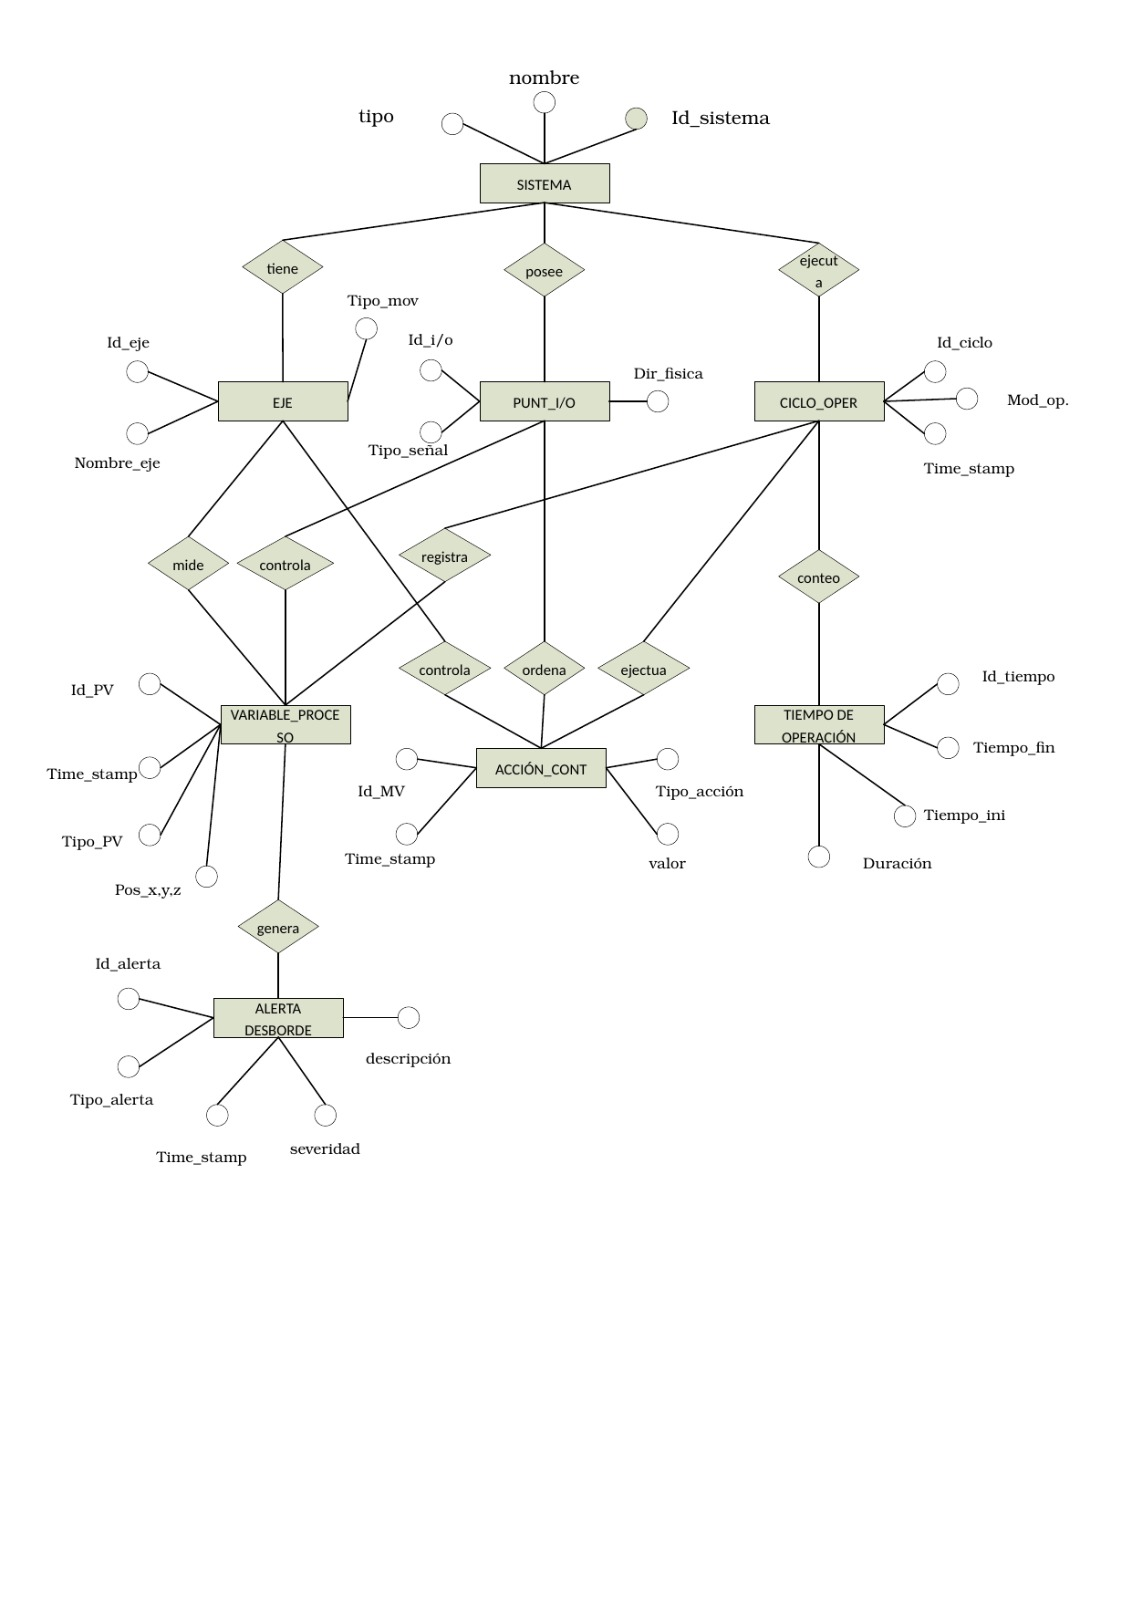
\includegraphics[width=0.55\linewidth, trim=0 360 0 0, clip]{modelo_er_preliminar.png}
\caption{Modelo E-R preliminar del equipo (\codigo{database/modelo/}).}
\end{figure}

El modelo preliminar ya tenía las entidades correctas, pero guardaba datos que rompen las formas normales: \emph{Pos\_x.y.z} (tres valores en un atributo), \emph{valor} de la acción de control (uno por eje), \emph{Duración} (se calcula con el inicio y el fin) y la alerta ligada a la variable en lugar del ciclo.

Para mostrar cada paso, se parte de la tabla plana que se obtendría guardando todo lo que la app ve en una sola planilla. \textbf{Los valores son ilustrativos}, no mediciones.

\begin{center}\scriptsize
\begin{tabular}{>{\ttfamily}l >{\ttfamily}l >{\ttfamily}l >{\ttfamily}l >{\ttfamily}l >{\ttfamily}l >{\ttfamily}l}
\toprule
instante & usuario & rol & modo & posicion ($\theta$, X, Y) & unidades & orden\\
\midrule
10:00:01 & ana & operador & red & 0, 20, 30 & °, mm, mm & mover $\theta$=45 X=80\\
10:00:02 & ana & operador & red & 12, 35, 30 & °, mm, mm & --\\
10:00:03 & luis & observador & red & 25, 51, 30 & °, mm, mm & mover (rechazada: rol)\\
\bottomrule
\end{tabular}
\end{center}

\subsection{Primera forma normal (1FN): valores atómicos}
\textbf{Regla}: cada celda tiene un solo valor y no hay grupos repetidos.

\textbf{Problema}: \emph{posicion} y \emph{unidades} tienen tres valores; \emph{orden} mezcla el tipo, los destinos y el resultado.

\textbf{Solución}: una fila por variable medida (\codigo{muestra}) y una fila por eje de destino (\codigo{orden\_parametro}).

\begin{center}\scriptsize
\begin{tabular}{>{\ttfamily}l >{\ttfamily}l >{\ttfamily}l >{\ttfamily}l >{\ttfamily}l >{\ttfamily}l >{\ttfamily}l}
\toprule
\underline{instante} & usuario & rol & modo & \underline{tag} & unidad & valor\\
\midrule
10:00:01 & ana & operador & red & ZI-101 & ° & 0\\
10:00:01 & ana & operador & red & ZI-102 & mm & 20\\
10:00:01 & ana & operador & red & ZI-103 & mm & 30\\
\multicolumn{7}{c}{\dots}\\
\bottomrule
\end{tabular}
\end{center}

\subsection{Segunda forma normal (2FN): dependencia de la clave completa}
\textbf{Regla}: estar en 1FN y que ningún atributo dependa solo de una parte de la clave.

\textbf{Problema}: la clave de la tabla anterior es (\emph{instante}, \emph{tag}). Pero \emph{unidad} depende solo de \emph{tag}, y \emph{usuario}, \emph{rol} y \emph{modo} dependen solo de \emph{instante} (del ciclo en curso). Son dependencias parciales: la unidad «mm» se repite en cada muestra y, si alguien la escribe mal una vez, la base queda inconsistente.

\textbf{Solución}: separar lo que depende del tag (\codigo{variable}: unidad, rango, clase) y lo que depende del ciclo (\codigo{ciclo\_operacion}: modo, inicio, fin). La muestra queda con su clave y su valor.

\begin{center}\scriptsize
\begin{tabular}{@{}l@{\hspace{6mm}}l@{\hspace{6mm}}l@{}}
\begin{tabular}[t]{>{\ttfamily}l >{\ttfamily}l >{\ttfamily}l}
\multicolumn{3}{l}{\textbf{variable}}\\\toprule
\underline{tag} & unidad & rango\\\midrule
ZI-101 & ° & $-263$..263\\ ZI-102 & mm & 0..170\\ ZI-103 & mm & 0..170\\\bottomrule
\end{tabular}
&
\begin{tabular}[t]{>{\ttfamily}l >{\ttfamily}l >{\ttfamily}l}
\multicolumn{3}{l}{\textbf{ciclo\_operacion}}\\\toprule
\underline{id} & modo & inicio\\\midrule
7 & red & 09:58:40\\\bottomrule
\end{tabular}
&
\begin{tabular}[t]{>{\ttfamily}l >{\ttfamily}l >{\ttfamily}l >{\ttfamily}l}
\multicolumn{4}{l}{\textbf{muestra}}\\\toprule
\underline{id} & ciclo & variable & valor\\\midrule
1 & 7 & ZI-101 & 0\\ 2 & 7 & ZI-102 & 20\\ 3 & 7 & ZI-103 & 30\\\bottomrule
\end{tabular}
\end{tabular}
\end{center}

En el script, la única tabla con clave compuesta es \codigo{orden\_parametro} (\codigo{orden\_id}, \codigo{eje\_id}), y su único atributo, \codigo{valor}, depende de los dos: el destino es de esa orden \emph{y} de ese eje. Por eso está en 2FN.

\subsection{Tercera forma normal (3FN): sin dependencias transitivas}
\textbf{Regla}: estar en 2FN y que ningún atributo no clave dependa de otro atributo no clave.

\textbf{Problemas} que quedaban:
\begin{itemize}
\item en la orden, \emph{rol} depende de \emph{usuario}, no de la orden (orden $\to$ usuario $\to$ rol);
\item la \emph{duración} del ciclo depende de \emph{inicio} y \emph{fin};
\item la severidad de una alarma depende del tipo de alarma, no del evento.
\end{itemize}

\textbf{Solución}: \codigo{rol} en su propia tabla, referida por \codigo{usuario.rol\_id}; la duración se calcula en la vista \codigo{v\_ciclo}; la severidad vive en el catálogo \codigo{alarma} y el evento solo dice cuándo ocurrió.

\begin{figure}[H]
\centering
\begin{tikzpicture}[node distance=3mm and 9mm, every node/.style={font=\scriptsize}]
\node[cajab, text width=3.2cm] (a) {\textbf{Tabla plana}\\posición en una celda\\unidad repetida\\rol en cada fila\\duración guardada};
\node[cajab, text width=3.2cm, right=of a] (b) {\textbf{1FN}\\una fila por variable\\una fila por eje de destino};
\node[cajab, text width=3.2cm, right=of b] (c) {\textbf{2FN}\\\codigo{variable} y \codigo{ciclo\_operacion} separadas de \codigo{muestra}};
\node[cajan, text width=3.2cm, right=of c] (d) {\textbf{3FN}\\\codigo{rol}, \codigo{alarma} como catálogos\\duración calculada (vista)};
\draw[flecha] (a) -- (b); \draw[flecha] (b) -- (c); \draw[flecha] (c) -- (d);
\end{tikzpicture}
\caption{Resumen de la normalización.}
\end{figure}

\subsection{Dependencias funcionales del modelo final}
\begin{center}\small
\begin{tabularx}{\linewidth}{>{\ttfamily\raggedright}p{4.6cm} >{\raggedright\arraybackslash}X}
\toprule
\textrm{\textbf{Determinante}} & \textbf{Determina}\\
\midrule
variable.id & tag\_isa, clase, nombre, unidad, rango\_min, rango\_max, eje\_id\\
variable.tag\_isa & lo mismo (clave candidata: es UNIQUE)\\
punto\_io.id & direccion, tag\_isa, tipo\_senal, descripcion, eje\_id\\
(punto\_io.sistema\_id, direccion) & lo mismo (clave candidata: UNIQUE)\\
muestra.id & ciclo\_id, variable\_id, instante, valor\\
ciclo\_operacion.id & sistema\_id, programa\_id, modo, inicio, fin\\
orden.id & ciclo\_id, usuario\_id, instante, tipo, aceptada, motivo\\
(orden\_id, eje\_id) & valor\\
usuario.id & nombre, rol\_id, clave\_hash, creado\_en\\
alarma.id & codigo, severidad, descripcion\\
\bottomrule
\end{tabularx}
\end{center}
En cada tabla todo determinante es una clave (primaria o candidata), así que el modelo también cumple la forma normal de Boyce-Codd (FNBC).

\subsection{Desnormalizaciones que no se hicieron}
\codigo{muestra} no repite \codigo{eje\_id} (se obtiene por la variable) ni \codigo{estado\_io} repite el tag (se obtiene por el punto). Cuesta una unión en cada consulta, pero las tablas de catálogo son tan chicas que PostgreSQL las mantiene en memoria.

% =====================================================================
\section{Correspondencia con los tags ISA-5.1}\label{sec:tags}

La guía 3 pide que el modelo refleje con fidelidad la nomenclatura de los lazos de control. Cada tag del P\&ID v2.0 (plano P\&ID-B4G-01) es una fila de la base:

\begin{figure}[H]
\centering
\begin{tikzpicture}[x=1cm, y=1cm, every node/.style={font=\scriptsize}]
\foreach \l/\nom [count=\i from 0] in {100/general,101/base,102/carro X,103/carro Y,104/garra} {
  \node[draw, thick, fill=naranja!12, minimum width=2.6cm, align=center] at (3*\i,0) {\textbf{Lazo \l}\\\nom};
}
\node[align=left, anchor=north] at (0,-0.8) {\ttfamily HS-100\\HS-100P\\ZY-100};
\node[align=left, anchor=north] at (3,-0.8) {\ttfamily ZS-101\\HS-101A/B\\ZY-101, ZY-101D\\ZI-101 \textrm{(PV)}\\SY-101 \textrm{(MV)}};
\node[align=left, anchor=north] at (6,-0.8) {\ttfamily ZSL/ZSH-102\\HS-102A/B\\ZY-102D, ZY-102K\\ZI-102 \textrm{(PV)}\\SY-100 \textrm{(MV)}};
\node[align=left, anchor=north] at (9,-0.8) {\ttfamily ZSL/ZSH-103\\HS-103A/B\\ZY-103D, ZY-103K\\ZI-103 \textrm{(PV)}};
\node[align=left, anchor=north] at (12,-0.8) {\ttfamily HS-104\\XY-104};
\node[draw, fill=gris, text width=13.5cm, align=left] at (6,-4.6) {\codigo{eje.lazo\_isa} guarda el número de lazo (101 a 104). Los tags de señales están en \codigo{punto\_io.tag\_isa} y los de variables continuas en \codigo{variable.tag\_isa}; ambos son UNIQUE, así que un tag no puede repetirse. El lazo 100 agrupa las señales sin eje propio (\codigo{eje\_id} = NULL).};
\end{tikzpicture}
\caption{Lazos del P\&ID v2.0 y los tags que la base carga en cada uno.}
\end{figure}

\begin{longtable}{>{\ttfamily}l >{\ttfamily}l l >{\raggedright}p{4.2cm} >{\raggedright\arraybackslash}p{3.4cm}}
\toprule
\textrm{\textbf{Tag}} & \textrm{\textbf{Dir.}} & \textbf{Tipo} & \textbf{Significado} & \textbf{Tabla / eje}\\
\midrule
\endhead
ZS-101 & I0.0 & DI & sensor inductivo de la base & \codigo{punto\_io} / Z\\
ZSL-102 & I0.1 & DI & final X atrás (origen) & \codigo{punto\_io} / X\\
ZSH-102 & I0.2 & DI & final X adelante & \codigo{punto\_io} / X\\
ZSL-103 & I0.3 & DI & final Y abajo (origen) & \codigo{punto\_io} / Y\\
ZSH-103 & I0.4 & DI & final Y arriba & \codigo{punto\_io} / Y\\
HS-100 & I0.5 & DI & selector manual / automático & \codigo{punto\_io} / --\\
HS-100P & I0.6 & DI & pulsador de paro & \codigo{punto\_io} / --\\
HS-104 & I0.7 & DI & garra / inicio & \codigo{punto\_io} / G\\
HS-101A/B & I1.0/I1.1 & DI & jog base $+$ / $-$ & \codigo{punto\_io} / Z\\
HS-102A/B & I1.2/I1.3 & DI & jog X adelante / atrás & \codigo{punto\_io} / X\\
HS-103A/B & I1.4/I1.5 & DI & jog Y arriba / abajo & \codigo{punto\_io} / Y\\
ZY-101 & Q0.0 & PTO & tren de pulsos de la base & \codigo{punto\_io} / Z\\
ZY-100 & Q0.1 & PTO & tren compartido X/Y & \codigo{punto\_io} / --\\
ZY-101D & Q0.2 & DO & dirección de la base & \codigo{punto\_io} / Z\\
ZY-102D & Q0.3 & DO & dirección X (0 = adelante) & \codigo{punto\_io} / X\\
ZY-103D & Q0.4 & DO & dirección Y (0 = arriba) & \codigo{punto\_io} / Y\\
ZY-102K & Q0.5 & DO & relé K1: tren al driver X & \codigo{punto\_io} / X\\
ZY-103K & Q0.6 & DO & relé K2: tren al driver Y & \codigo{punto\_io} / Y\\
XY-104 & Q0.7 & DO & solenoide de la garra & \codigo{punto\_io} / G\\
ZI-101 & -- & PV & posición de la base (°) & \codigo{variable} / Z\\
ZI-102 & -- & PV & posición del carro X (mm) & \codigo{variable} / X\\
ZI-103 & -- & PV & posición del carro Y (mm) & \codigo{variable} / Y\\
SY-101 & -- & MV & frecuencia del tren de la base (Hz) & \codigo{variable} / Z\\
SY-100 & -- & MV & frecuencia del tren X/Y (Hz) & \codigo{variable} / X\\
\bottomrule
\end{longtable}
\nota{SY-100 está asociada al eje X porque \codigo{variable.eje\_id} es obligatorio, pero el tren es compartido: en cada instante mueve el eje que eligieron K1 o K2. Para saber qué eje movió, se cruza con el estado de ZY-102K y ZY-103K en \codigo{estado\_io}.}

% =====================================================================
\section{El script SQL}\label{sec:script}

El script \archivo{scripts/brazo\_4gdl.sql} crea todo en una sola transacción (\codigo{BEGIN} \dots\ \codigo{COMMIT}): si una sentencia falla, no queda nada a medias.

\begin{center}\small
\begin{tabularx}{\linewidth}{>{\raggedright}p{3.2cm} >{\raggedright\arraybackslash}X}
\toprule
\textbf{Parte} & \textbf{Contenido}\\
\midrule
DDL · catálogos & \codigo{sistema}, \codigo{eje}, \codigo{punto\_io}, \codigo{variable}, \codigo{programa\_plc}, \codigo{alarma}\\
DDL · seguridad & \codigo{rol}, \codigo{usuario}, \codigo{sesion}\\
DDL · operación & \codigo{ciclo\_operacion}, \codigo{muestra}, \codigo{estado\_io}, \codigo{orden}, \codigo{orden\_parametro}, \codigo{evento\_alarma}\\
Índices & \codigo{muestra(variable\_id, instante)} y \codigo{estado\_io(punto\_id, instante)}\\
Reglas & claves foráneas con \codigo{ON DELETE RESTRICT ON UPDATE CASCADE}; función \codigo{verificar\_limites\_variables()} y trigger \codigo{muestra\_en\_rango}\\
Vistas & \codigo{v\_ciclo} (duración) y \codigo{v\_ultima\_posicion}\\
DML · datos de la planta & 1 sistema, 4 ejes, 22 señales, 5 variables, 3 programas, 9 alarmas, 2 roles\\
\bottomrule
\end{tabularx}
\end{center}

\begin{lstlisting}[style=sql, caption={Ejemplo de DDL: la tabla de telemetría y su índice.}]
CREATE TABLE muestra (                                   -- telemetría de variables continuas
    id          BIGSERIAL PRIMARY KEY,
    ciclo_id    BIGINT           NOT NULL REFERENCES ciclo_operacion(id),
    variable_id SMALLINT         NOT NULL REFERENCES variable(id),
    instante    TIMESTAMPTZ      NOT NULL,
    valor       DOUBLE PRECISION NOT NULL
);
CREATE INDEX muestra_variable_instante ON muestra (variable_id, instante);
\end{lstlisting}

\paragraph{Por qué ese índice.} Casi todas las consultas del dashboard piden «la variable $V$ entre $t_1$ y $t_2$» o «el último valor de $V$». Un índice B-tree con \codigo{variable\_id} primero y \codigo{instante} después deja todas las muestras de una variable juntas y ordenadas por tiempo, así que PostgreSQL encuentra el intervalo sin recorrer la tabla. El orden de las columnas importa: al revés, el índice serviría para buscar por tiempo, pero mezclaría todas las variables.

\paragraph{Validación.} Se ejecutó en PostgreSQL 16.2 el 12/11/2026, en la PC de desarrollo del equipo: la base se crea sin errores, las 7 pruebas de \codigo{prueba\_reglas.sql} dan «correcta», se cargaron 18\,000 muestras sintéticas (\codigo{datos\_sinteticos.sql}) y las 14 consultas del dashboard responden; el plan de ejecución confirma que el índice por marca de tiempo se usa. Todo queda en \codigo{database/scripts/registro\_ejecucion.txt}. Falta repetirlo en la PC del laboratorio.

% =====================================================================
\section{Reglas de integridad}\label{sec:reglas}

La guía 1 pide que la base impida datos nulos o fuera de rango, y la guía 5, que un trigger aísle la variable fuera de límite, registre la alerta y cambie el estado de la planta. Hay cinco barreras, de la más simple a la más específica:

\begin{center}\small
\begin{tabularx}{\linewidth}{>{\raggedright}p{2.8cm} >{\raggedright}X >{\raggedright\arraybackslash}p{4.4cm}}
\toprule
\textbf{Mecanismo} & \textbf{Qué impide} & \textbf{Ejemplo}\\
\midrule
\codigo{NOT NULL} & dejar vacío un dato obligatorio & una muestra sin valor o sin instante\\
\codigo{CHECK} & valores fuera de una lista o rango fijo & \codigo{modo = 'turbo'}; severidad 5; \codigo{fin < inicio}\\
\codigo{REFERENCES} (FK) & referencias a filas que no existen; borrar un dato con historial (\codigo{ON DELETE RESTRICT}) & una muestra de la variable 999; borrar ZI-102 con muestras\\
\codigo{UNIQUE} & duplicados & dos señales con el tag ZS-101\\
Trigger & valores fuera del rango de \emph{esa} variable: los descarta, registra la alerta y saca la planta de operación & X = 250 mm (el carro llega a 170)\\
\bottomrule
\end{tabularx}
\end{center}

El rango no se puede escribir como un \codigo{CHECK} de la tabla \codigo{muestra}, porque depende de otra tabla (\codigo{variable}): por eso es un trigger. Todas las claves foráneas declaran \codigo{ON DELETE RESTRICT ON UPDATE CASCADE} (guía 4): no se puede borrar un catálogo que ya tiene historial, y un cambio de clave se propaga. La única excepción es \codigo{orden\_parametro}, que se borra con su orden (\codigo{ON DELETE CASCADE}).

\begin{figure}[H]
\centering
\begin{tikzpicture}[node distance=5mm, every node/.style={font=\scriptsize}]
\node[cajab] (i) {\codigo{INSERT} o \codigo{UPDATE} en \codigo{muestra}};
\node[cajab, below=of i] (n) {NOT NULL, FK: ¿valor, ciclo y variable válidos?};
\node[cajab, below=of n] (t) {trigger \codigo{BEFORE}: busca \codigo{rango\_min} y \codigo{rango\_max} de la variable};
\node[diamond, draw, aspect=2.4, fill=naranja!12, below=of t, align=center, inner sep=1pt] (d) {¿mín $\le$ valor $\le$ máx?};
\node[cajan, below left=6mm and 6mm of d] (ok) {la fila se guarda};
\node[caja, fill=rojo!12, below right=6mm and 6mm of d, text width=5.6cm, align=left] (no) {1. alerta \codigo{limite\_variable} en \codigo{evento\_alarma}\\2. \codigo{sistema.en\_operacion = false}\\3. \codigo{RETURN NULL}: la muestra no se guarda};
\draw[flecha] (i) -- (n); \draw[flecha] (n) -- (t); \draw[flecha] (t) -- (d);
\draw[flecha] (d) -| node[above, pos=0.2]{sí} (ok); \draw[flecha] (d) -| node[above, pos=0.2]{no} (no);
\end{tikzpicture}
\caption{Camino de una muestra hasta la tabla.}
\end{figure}

\begin{lstlisting}[style=sql, caption={Trigger de seguridad (\codigo{brazo\_4gdl.sql}).}]
CREATE FUNCTION verificar_limites_variables() RETURNS trigger AS $$
DECLARE
    r variable%ROWTYPE;
BEGIN
    SELECT * INTO r FROM variable WHERE id = NEW.variable_id;
    IF NEW.valor < r.rango_min OR NEW.valor > r.rango_max THEN
        INSERT INTO evento_alarma (alarma_id, ciclo_id, instante, activa, detalle)
        SELECT a.id, NEW.ciclo_id, clock_timestamp(), true,
               format('%s = %s %s fuera de [%s, %s]', r.tag_isa, NEW.valor, r.unidad, r.rango_min, r.rango_max)
        FROM alarma a WHERE a.codigo = 'limite_variable';
        UPDATE sistema SET en_operacion = false
        WHERE id = (SELECT sistema_id FROM ciclo_operacion WHERE id = NEW.ciclo_id);
        RAISE WARNING 'muestra descartada: % = % % fuera de [%, %]',
            r.tag_isa, NEW.valor, r.unidad, r.rango_min, r.rango_max;
        RETURN NULL;
    END IF;
    RETURN NEW;
END;
$$ LANGUAGE plpgsql;
CREATE TRIGGER muestra_en_rango BEFORE INSERT OR UPDATE ON muestra
    FOR EACH ROW EXECUTE FUNCTION verificar_limites_variables();
\end{lstlisting}

\paragraph{Por qué \codigo{RETURN NULL} y no \codigo{RAISE EXCEPTION}.} Una excepción deshace toda la transacción, incluida la alerta que el trigger acaba de registrar: la falla quedaría sin rastro. Al devolver \codigo{NULL}, PostgreSQL omite solo la fila de la muestra y conserva la alerta y el cambio de estado. \codigo{clock\_timestamp()} da la hora real del instante de la inserción, en UTC y con microsegundos (\codigo{now()} daría la hora de inicio de la transacción).

\paragraph{Nombres de la guía 5.} La guía nombra las tablas \codigo{historico\_telemetria} y \codigo{registro\_alertas}; en este modelo son \codigo{muestra} y \codigo{evento\_alarma}, que ya existían con esa función en el modelo 3FN. El trigger sí lleva el nombre que pide la guía.

El script \archivo{scripts/prueba\_reglas.sql} prueba un caso válido, las cinco barreras y la restricción de borrado dentro de una transacción que se deshace al final (no deja datos). Por cada caso imprime «prueba $n$ correcta» o «FALLÓ»:
\begin{enumerate}
\item una muestra de 85 mm en ZI-102 entra;
\item una de 250 mm la descarta el trigger, que registra la alerta y deja la planta fuera de operación;
\item una sin valor la rechaza NOT NULL;
\item un ciclo en modo «turbo» lo rechaza CHECK;
\item una muestra de una variable inexistente la rechaza la clave foránea;
\item un tag repetido lo rechaza UNIQUE;
\item borrar la variable ZI-102, que ya tiene muestras, lo impide \codigo{ON DELETE RESTRICT}.
\end{enumerate}

\subsection*{Vistas}
\begin{itemize}
\item \codigo{v\_ciclo}: cada ciclo con su programa y su duración \codigo{fin - inicio} (o hasta ahora si sigue abierto). La duración no se guarda: es la consecuencia de la 3FN.
\item \codigo{v\_ultima\_posicion}: el último valor de cada PV, usando \codigo{DISTINCT ON}, que aprovecha el índice de \codigo{muestra}.
\end{itemize}

% =====================================================================
\section{Flujo de datos}\label{sec:flujo}

\subsection{Diagrama de contexto (DFD nivel 0)}
\begin{figure}[H]
\centering
\begin{tikzpicture}[x=1cm, y=1cm, every node/.style={font=\scriptsize}]
\node[proc, minimum size=24mm] (s) at (0,0) {\textbf{0}\\Gemelo digital\\+ base\\\codigo{brazo4gdl}};
\node[extd] (plc) at (-6.2,0) {PLC S7-200\\(planta)};
\node[extd] (op) at (-4.2,3.2) {Operador\\(local o remoto)};
\node[extd] (ob) at (4.2,3.2) {Observador};
\node[extd] (doc) at (6.2,0) {Docente / analista\\(dashboard)};
\draw[flecha] ([yshift=2mm]plc.east) -- node[above, etiq]{E/S, pulsos, posición} ([yshift=2mm]s.west);
\draw[flecha] ([yshift=-2mm]s.west) -- node[below, etiq]{órdenes (VB1100...)} ([yshift=-2mm]plc.east);
\draw[flecha] ([xshift=-3mm]op.south) -- node[left, etiq, pos=0.45]{credenciales,\\órdenes} (s.north west);
\draw[flecha] (s.155) -- node[right, etiq, pos=0.7]{estado, 3D} ([xshift=6mm]op.south);
\draw[flecha] ([xshift=3mm]ob.south) -- node[right, etiq, pos=0.45]{credenciales} (s.north east);
\draw[flecha] (s.25) -- node[left, etiq, pos=0.7]{estado (lectura)} ([xshift=-6mm]ob.south);
\draw[flecha] (s.east) -- node[above, etiq]{KPIs, historial} (doc.west);
\end{tikzpicture}
\caption{DFD nivel 0: actores externos y datos que intercambian con el sistema.}
\end{figure}

\subsection{DFD nivel 1}
\begin{figure}[H]
\centering
\begin{tikzpicture}[x=0.95cm, y=1cm, every node/.style={font=\scriptsize},
  dato/.style={rectangle split, rectangle split horizontal, rectangle split parts=2, draw, thick, fill=white, font=\scriptsize, inner sep=3pt}]
\node[extd] (plc) at (0,5) {PLC};
\node[extd] (us) at (0,-1) {Operador /\\observador};
\node[extd] (doc) at (16.9,1.8) {Dashboard};
\node[proc] (p1) at (3.8,5) {\textbf{1}\\Adquirir\\por PPI};
\node[proc] (p2) at (3.8,-1) {\textbf{2}\\Autenticar};
\node[proc] (p3) at (8,1.8) {\textbf{3}\\Validar y\\ejecutar\\órdenes};
\node[proc] (p4) at (8,5) {\textbf{4}\\Registrar};
\node[proc] (p5) at (12.4,1.8) {\textbf{5}\\Consultar\\KPIs};
\node[dato] (d1) at (12.4,5.9) {\textbf{D1}\nodepart{two}muestra, estado\_io};
\node[dato] (d2) at (12.4,4.5) {\textbf{D2}\nodepart{two}ciclo, orden};
\node[dato] (d3) at (12.4,-1) {\textbf{D3}\nodepart{two}evento\_alarma};
\node[dato] (d4) at (3.8,-3) {\textbf{D4}\nodepart{two}usuario, sesion};
\node[dato] (d5) at (8,-1) {\textbf{D5}\nodepart{two}catálogo};
\draw[flecha] (plc) -- node[above, etiq]{tramas} (p1);
\draw[flecha] (p1) -- node[above, etiq]{estado} (p4);
\draw[flecha] (p1) -- node[below left, etiq, pos=0.45]{estado} (p3);
\draw[flecha] (p3.north west) |- ++(0,0.9) -| node[right, etiq, pos=0.75]{escritura VB} (plc.south);
\draw[flecha] (us) -- node[below, etiq]{usuario, clave} (p2);
\draw[flecha] (p2) -- node[right, etiq]{intento} (d4);
\draw[flecha] (p2) -- node[below right, etiq, pos=0.4]{rol} (p3);
\draw[flecha] (us.north) |- node[above, etiq, pos=0.75]{órdenes} (p3.west);
\draw[flecha] (d5) -- node[right, etiq]{rangos} (p3);
\draw[flecha] (p3) -- node[right, etiq]{orden, motivo} (p4);
\draw[flecha] (p4) -- (d1.west); \draw[flecha] (p4) -- (d2.west);
\draw[flecha] (p3) -- node[above, etiq, sloped]{alarma} (d3.west);
\draw[flecha] (d2) -- (p5);
\draw[flecha] (d1.east) -- ++(0.5,0) |- (p5.35);
\draw[flecha] (d3) -- (p5);
\draw[flecha] (p5.-10) -- node[below, etiq]{tablas, gráficos} (doc.west |- p5.-10);
\end{tikzpicture}
\caption{DFD nivel 1: procesos (círculos), almacenes de datos D1 a D5 y flujos. Los procesos 1 a 3 ya existen en la app; 4 y 5 son la integración propuesta.}
\end{figure}

\subsection{Secuencia de inserción propuesta}
La app lee el PLC en un bucle continuo (cada lectura PPI de 9600 bit/s tarda unos 155~ms). Guardar cada lectura llenaría la base sin aportar información, así que se propone:
\begin{itemize}
\item \codigo{muestra}: una fila por segundo y por variable (5 variables $\Rightarrow$ 5 filas/s);
\item \codigo{estado\_io}: solo cuando una señal cambia (flanco);
\item \codigo{orden}, \codigo{sesion}, \codigo{evento\_alarma}: en el momento en que ocurren;
\item \codigo{ciclo\_operacion}: una fila al elegir un modo en el menú; se cierra (\codigo{fin}) al cambiar de modo o salir.
\end{itemize}

\begin{figure}[H]
\centering
\begin{tikzpicture}[x=1cm, y=-0.62cm, every node/.style={font=\scriptsize}]
\foreach \x/\n in {0/PLC, 4/{App (bucle PPI)}, 8.5/{Registrador (hilo)}, 13/PostgreSQL} {
  \node[draw, fill=gris, minimum width=2.6cm] at (\x,0) {\n};
  \draw[dashed, black!50] (\x,0.6) -- (\x,13);
}
\draw[flecha] (4,1.5) -- node[above]{leer E/S y posición} (0,1.5);
\draw[flecha] (0,2.5) -- node[above]{respuesta (155 ms)} (4,2.5);
\draw[flecha] (4,3.5) -- node[above]{estado en cola} (8.5,3.5);
\node[align=left, anchor=west] at (8.7,4.5) {¿pasó 1 s? / ¿cambió una señal?};
\draw[flecha] (8.5,5.5) -- node[above]{\codigo{INSERT INTO muestra} (5 filas)} (13,5.5);
\draw[flecha] (8.5,6.5) -- node[above]{\codigo{INSERT INTO estado\_io} (flancos)} (13,6.5);
\node[align=left, anchor=west, text width=3.4cm] at (13.2,7.2) {trigger de rango, FK, NOT NULL};
\draw[flecha, dashed] (13,8.2) -- node[above]{OK o excepción} (8.5,8.2);
\draw[flecha] (4,9.5) -- node[above]{orden del usuario} (8.5,9.5);
\draw[flecha] (8.5,10.5) -- node[above]{\codigo{INSERT INTO orden} + \codigo{orden\_parametro}} (13,10.5);
\draw[flecha] (4,11.7) -- node[above]{escribir VB1100...} (0,11.7);
\end{tikzpicture}
\caption{Secuencia propuesta: la inserción va en un hilo aparte para que una base lenta o caída no frene la lectura del PLC.}
\end{figure}

\nota{\textbf{Por qué un hilo aparte.} Si el servidor PostgreSQL no responde, el registrador encola las filas y reintenta; el bucle PPI y el watchdog del PLC nunca esperan a la base. Así la seguridad del brazo no depende de la base de datos.}

\subsection{De la app a las tablas}
\begin{center}\small
\begin{tabularx}{\linewidth}{>{\raggedright}p{6cm} >{\raggedright\arraybackslash}X}
\toprule
\textbf{Dato que ya produce la app} & \textbf{Tabla}\\
\midrule
cambio de modo en el menú & \codigo{ciclo\_operacion}\\
\codigo{/api/estado}: \codigo{theta\_deg}, \codigo{sX\_mm}, \codigo{sY\_mm} & \codigo{muestra} (ZI-101, ZI-102, ZI-103)\\
\codigo{/api/estado}: entradas y salidas & \codigo{estado\_io} (solo los cambios)\\
línea \codigo{orden mover \{...\} (usuario)} del registro & \codigo{orden} + \codigo{orden\_parametro}\\
línea \codigo{RECHAZADO ...} & \codigo{orden} con \codigo{aceptada = false} y su motivo\\
error del PLC, pérdida de comunicación, watchdog & \codigo{evento\_alarma}\\
\codigo{usuarios.json} & \codigo{usuario} y \codigo{rol} (mismo hash PBKDF2)\\
líneas \codigo{ingreso de ...} / \codigo{ingreso fallido} & \codigo{sesion}\\
\bottomrule
\end{tabularx}
\end{center}

% =====================================================================
\section{De los mockups a las consultas}\label{sec:mockups}

La guía 2 pide justificar cómo los mockups definen lo que la base debe guardar. Cada elemento de los dos entornos diseñados (interfaz local y dashboard web) se responde con una tabla y una consulta de \archivo{scripts/consultas\_kpi.sql}:

\begin{figure}[H]
\centering
\includegraphics[page=3, width=0.48\linewidth]{lab2_mockups_y_organigrama.pdf}\hfill
\includegraphics[page=4, width=0.48\linewidth]{lab2_mockups_y_organigrama.pdf}
\caption{Mockups del laboratorio 2: interfaz local (izquierda) y dashboard web (derecha).}
\end{figure}

\begin{longtable}{>{\raggedright}p{4.5cm} >{\raggedright}p{5.2cm} >{\raggedright\arraybackslash}p{4.6cm}}
\toprule
\textbf{Elemento del mockup} & \textbf{De dónde sale} & \textbf{Consulta}\\
\midrule
\endhead
\multicolumn{3}{l}{\textit{Dashboard web}}\\
Reloj y estado «En línea» & ciclo con \codigo{fin IS NULL} & consulta 1\\
Tiempo encendido & suma de duraciones de \codigo{v\_ciclo} & consulta 2\\
Ciclos completados & órdenes \codigo{iniciar} aceptadas & consulta 3\\
Tren de pulsos (progreso) & última muestra de SY-100 y SY-101 & consulta 4\\
Bit de dirección y bit habilitador & último estado de Q0.2 a Q0.6 en \codigo{estado\_io} (ver nota) & consulta 5\\
Lecturas de sensores en tiempo real & último estado de I0.0 a I0.4 & consulta 6\\
Historial de sesiones & \codigo{sesion} con el rol del usuario & consulta 9\\
Gráficos históricos & serie de tiempo de una PV & consulta 8\\
\midrule
\multicolumn{3}{l}{\textit{Interfaz local}}\\
Selector de modo manual / auto & señal HS-100 (I0.5) & consulta 6 cambiando las direcciones\\
Parada de emergencia & orden \codigo{emergencia} y alarma \codigo{paro} & consultas 11 y 13\\
Botonera: reiniciar, iniciar, detener & órdenes \codigo{rearmar}, \codigo{iniciar}, \codigo{detener} & consulta 13\\
Seis botones de movimiento & órdenes \codigo{mover} con destinos por eje & consulta 14\\
Botón de pinza & orden \codigo{garra} y señal XY-104 & consultas 5 y 13\\
Sensores 1--4 e inductivo & ZSL/ZSH-102/103 y ZS-101 & consulta 6\\
Indicador de estado del sistema & alarmas activas & consulta 11\\
Posición actual & vista \codigo{v\_ultima\_posicion} & consulta 7\\
\bottomrule
\end{longtable}

\nota{\textbf{Bit habilitador.} El mockup muestra un bit «habilitador», pero en el esquema eléctrico v2.0 la entrada ENA de los drivers está libre (siempre habilitados): no hay una señal del PLC que guardar. Lo más parecido son los relés K1 y K2 (ZY-102K, ZY-103K), que eligen a qué driver llega el tren de pulsos; la consulta 5 los incluye.}

% =====================================================================
\section{Consultas de ejemplo}\label{sec:consultas}

\begin{lstlisting}[style=sql, caption={Tiempo encendido por día y por modo (consulta 2).}]
SELECT date_trunc('day', inicio) AS dia, modo,
       round(extract(epoch FROM sum(duracion)) / 3600.0, 2) AS horas
FROM v_ciclo
GROUP BY 1, 2
ORDER BY 1 DESC, 2;
\end{lstlisting}

\begin{lstlisting}[style=sql, caption={Alarmas activas en este momento (consulta 11).}]
SELECT a.codigo, a.severidad, ult.instante, ult.detalle
FROM (SELECT DISTINCT ON (alarma_id) alarma_id, activa, instante, detalle
      FROM evento_alarma ORDER BY alarma_id, instante DESC) ult
JOIN alarma a ON a.id = ult.alarma_id
WHERE ult.activa
ORDER BY a.severidad DESC, ult.instante;
\end{lstlisting}

\begin{lstlisting}[style=sql, caption={La 1FN se deshace solo al mostrar: destinos de cada orden en una fila (consulta 14).}]
SELECT o.id, o.instante,
       max(p.valor) FILTER (WHERE e.codigo = 'Z') AS theta_deg,
       max(p.valor) FILTER (WHERE e.codigo = 'X') AS x_mm,
       max(p.valor) FILTER (WHERE e.codigo = 'Y') AS y_mm
FROM orden o
JOIN orden_parametro p ON p.orden_id = o.id
JOIN eje e ON e.id = p.eje_id
WHERE o.tipo = 'mover'
GROUP BY o.id, o.instante
ORDER BY o.instante DESC;
\end{lstlisting}

\begin{lstlisting}[style=sql, caption={Seguridad: IP con tres o más ingresos fallidos en el último día (consulta 10).}]
SELECT ip, count(*) AS fallidos
FROM sesion
WHERE NOT exito AND instante > now() - interval '1 day'
GROUP BY ip
HAVING count(*) >= 3
ORDER BY 2 DESC;
\end{lstlisting}

% =====================================================================
\section{Diccionario de datos}\label{sec:diccionario}
Generado automáticamente desde el script con \codigo{generar\_diccionario.py}, para que nunca quede desactualizado. PK: clave primaria; FK: clave foránea; UQ: único; Nulo: si la columna acepta NULL.
{\small
% Generado por generar_diccionario.py a partir de ../scripts/brazo_4gdl.sql: no editar a mano
\subsection*{\codigo{sistema}}
\begin{longtable}{>{\ttfamily\raggedright}p{2.6cm} >{\ttfamily\raggedright}p{2.5cm} c >{\raggedright\footnotesize}p{3.6cm} >{\raggedright\arraybackslash}p{4.5cm}}
\toprule \textrm{\textbf{Columna}} & \textrm{\textbf{Tipo}} & \textbf{Nulo} & \textbf{Restricción} & \textbf{Descripción}\\ \midrule
id & SMALLSERIAL & no & PK & identificador (clave sustituta)\\
nombre & VARCHAR(60) & no & UQ & nombre de la planta\\
tipo & VARCHAR(40) & no &  & tipo de planta\\
plc & VARCHAR(60) & no &  & PLC que la controla\\
en\_operacion & BOOLEAN & no & DEFAULT true & false: un trigger detectó una variable fuera de límite\\
\bottomrule \end{longtable}
\subsection*{\codigo{eje}}
\begin{longtable}{>{\ttfamily\raggedright}p{2.6cm} >{\ttfamily\raggedright}p{2.5cm} c >{\raggedright\footnotesize}p{3.6cm} >{\raggedright\arraybackslash}p{4.5cm}}
\toprule \textrm{\textbf{Columna}} & \textrm{\textbf{Tipo}} & \textbf{Nulo} & \textbf{Restricción} & \textbf{Descripción}\\ \midrule
id & SMALLSERIAL & no & PK & identificador (clave sustituta)\\
sistema\_id & SMALLINT & no & FK$\to$sistema & \\
codigo & CHAR(1) & no &  & Z (base), X, Y, G (garra)\\
nombre & VARCHAR(40) & no &  & nombre del grado de libertad\\
tipo\_mov & VARCHAR(12) & no & CHECK & rotacional, lineal o binario\\
unidad & VARCHAR(8) & no &  & unidad de la posición\\
pulsos\_unidad & NUMERIC(10,4) & sí &  & NULL para la garra\\
lazo\_isa & SMALLINT & no &  & número de lazo ISA (101 a 104)\\
\midrule \multicolumn{5}{l}{\small Restricciones de tabla: \texttt{UNIQUE (sistema\_id, codigo)}}\\
\bottomrule \end{longtable}
\subsection*{\codigo{punto\_io}}
\begin{longtable}{>{\ttfamily\raggedright}p{2.6cm} >{\ttfamily\raggedright}p{2.5cm} c >{\raggedright\footnotesize}p{3.6cm} >{\raggedright\arraybackslash}p{4.5cm}}
\toprule \textrm{\textbf{Columna}} & \textrm{\textbf{Tipo}} & \textbf{Nulo} & \textbf{Restricción} & \textbf{Descripción}\\ \midrule
id & SMALLSERIAL & no & PK & identificador (clave sustituta)\\
sistema\_id & SMALLINT & no & FK$\to$sistema & \\
eje\_id & SMALLINT & sí & FK$\to$eje & NULL: señal general del panel\\
direccion & VARCHAR(8) & no &  & I0.1, Q0.5 ...\\
tag\_isa & VARCHAR(16) & no & UQ & tag ISA-5.1 de la señal\\
tipo\_senal & VARCHAR(4) & no & CHECK & DI, DO o PTO\\
descripcion & VARCHAR(120) & no &  & qué hace la señal\\
\midrule \multicolumn{5}{l}{\small Restricciones de tabla: \texttt{UNIQUE (sistema\_id, direccion)}}\\
\bottomrule \end{longtable}
\subsection*{\codigo{variable}}
\begin{longtable}{>{\ttfamily\raggedright}p{2.6cm} >{\ttfamily\raggedright}p{2.5cm} c >{\raggedright\footnotesize}p{3.6cm} >{\raggedright\arraybackslash}p{4.5cm}}
\toprule \textrm{\textbf{Columna}} & \textrm{\textbf{Tipo}} & \textbf{Nulo} & \textbf{Restricción} & \textbf{Descripción}\\ \midrule
id & SMALLSERIAL & no & PK & identificador (clave sustituta)\\
eje\_id & SMALLINT & no & FK$\to$eje & \\
tag\_isa & VARCHAR(16) & no & UQ & tag ISA-5.1 de la variable\\
clase & CHAR(2) & no & CHECK & PV, MV o DV\\
nombre & VARCHAR(80) & no &  & nombre de la magnitud\\
unidad & VARCHAR(8) & no &  & unidad de ingeniería\\
rango\_min & DOUBLE PRECISION & no &  & mínimo admisible (lo usa el trigger)\\
rango\_max & DOUBLE PRECISION & no &  & máximo admisible (lo usa el trigger)\\
\midrule \multicolumn{5}{l}{\small Restricciones de tabla: \texttt{CHECK (rango\_min < rango\_max)}}\\
\bottomrule \end{longtable}
\subsection*{\codigo{programa\_plc}}
\begin{longtable}{>{\ttfamily\raggedright}p{2.6cm} >{\ttfamily\raggedright}p{2.5cm} c >{\raggedright\footnotesize}p{3.6cm} >{\raggedright\arraybackslash}p{4.5cm}}
\toprule \textrm{\textbf{Columna}} & \textrm{\textbf{Tipo}} & \textbf{Nulo} & \textbf{Restricción} & \textbf{Descripción}\\ \midrule
id & SMALLSERIAL & no & PK & identificador (clave sustituta)\\
nombre & VARCHAR(40) & no & UQ & nombre del programa ladder\\
perfil\_app & VARCHAR(12) & no & UQ & gemelo, cargado, monitor\\
firma & VARCHAR(40) & sí &  & valores de memoria que lo identifican\\
descripcion & VARCHAR(160) & sí &  & qué hace\\
\bottomrule \end{longtable}
\subsection*{\codigo{alarma}}
\begin{longtable}{>{\ttfamily\raggedright}p{2.6cm} >{\ttfamily\raggedright}p{2.5cm} c >{\raggedright\footnotesize}p{3.6cm} >{\raggedright\arraybackslash}p{4.5cm}}
\toprule \textrm{\textbf{Columna}} & \textrm{\textbf{Tipo}} & \textbf{Nulo} & \textbf{Restricción} & \textbf{Descripción}\\ \midrule
id & SMALLSERIAL & no & PK & identificador (clave sustituta)\\
codigo & VARCHAR(24) & no & UQ & código corto de la alarma\\
severidad & SMALLINT & no & CHECK & 1 aviso, 2 falla, 3 crítica\\
descripcion & VARCHAR(160) & no &  & significado\\
\bottomrule \end{longtable}
\subsection*{\codigo{rol}}
\begin{longtable}{>{\ttfamily\raggedright}p{2.6cm} >{\ttfamily\raggedright}p{2.5cm} c >{\raggedright\footnotesize}p{3.6cm} >{\raggedright\arraybackslash}p{4.5cm}}
\toprule \textrm{\textbf{Columna}} & \textrm{\textbf{Tipo}} & \textbf{Nulo} & \textbf{Restricción} & \textbf{Descripción}\\ \midrule
id & SMALLSERIAL & no & PK & identificador (clave sustituta)\\
nombre & VARCHAR(16) & no & UQ & observador u operador\\
\bottomrule \end{longtable}
\subsection*{\codigo{usuario}}
\begin{longtable}{>{\ttfamily\raggedright}p{2.6cm} >{\ttfamily\raggedright}p{2.5cm} c >{\raggedright\footnotesize}p{3.6cm} >{\raggedright\arraybackslash}p{4.5cm}}
\toprule \textrm{\textbf{Columna}} & \textrm{\textbf{Tipo}} & \textbf{Nulo} & \textbf{Restricción} & \textbf{Descripción}\\ \midrule
id & SERIAL & no & PK & identificador (clave sustituta)\\
nombre & VARCHAR(32) & no & UQ & nombre de ingreso\\
rol\_id & SMALLINT & no & FK$\to$rol & rol del usuario\\
clave\_hash & VARCHAR(200) & no &  & PBKDF2, igual que usuarios.json de la app\\
creado\_en & TIMESTAMPTZ & no & DEFAULT now() & fecha de alta\\
\bottomrule \end{longtable}
\subsection*{\codigo{sesion}}
\begin{longtable}{>{\ttfamily\raggedright}p{2.6cm} >{\ttfamily\raggedright}p{2.5cm} c >{\raggedright\footnotesize}p{3.6cm} >{\raggedright\arraybackslash}p{4.5cm}}
\toprule \textrm{\textbf{Columna}} & \textrm{\textbf{Tipo}} & \textbf{Nulo} & \textbf{Restricción} & \textbf{Descripción}\\ \midrule
id & BIGSERIAL & no & PK & identificador (clave sustituta)\\
usuario\_id & INTEGER & sí & FK$\to$usuario & NULL: usuario inexistente\\
nombre\_usado & VARCHAR(32) & no &  & nombre que se escribió\\
ip & INET & no &  & dirección IP del equipo\\
instante & TIMESTAMPTZ & no & DEFAULT now() & momento del intento\\
exito & BOOLEAN & no &  & ingreso aceptado o no\\
fin & TIMESTAMPTZ & sí &  & cierre de la sesión\\
\bottomrule \end{longtable}
\subsection*{\codigo{ciclo\_operacion}}
\begin{longtable}{>{\ttfamily\raggedright}p{2.6cm} >{\ttfamily\raggedright}p{2.5cm} c >{\raggedright\footnotesize}p{3.6cm} >{\raggedright\arraybackslash}p{4.5cm}}
\toprule \textrm{\textbf{Columna}} & \textrm{\textbf{Tipo}} & \textbf{Nulo} & \textbf{Restricción} & \textbf{Descripción}\\ \midrule
id & BIGSERIAL & no & PK & identificador (clave sustituta)\\
sistema\_id & SMALLINT & no & FK$\to$sistema & planta\\
programa\_id & SMALLINT & sí & FK$\to$programa\_plc & programa reconocido en el PLC\\
modo & VARCHAR(12) & no & CHECK & simulacion, local o red\\
inicio & TIMESTAMPTZ & no & DEFAULT now() & inicio del ciclo\\
fin & TIMESTAMPTZ & sí &  & fin (NULL: en curso)\\
\midrule \multicolumn{5}{l}{\small Restricciones de tabla: \texttt{CHECK (fin IS NULL OR fin >= inicio)}}\\
\bottomrule \end{longtable}
\subsection*{\codigo{muestra}}
\begin{longtable}{>{\ttfamily\raggedright}p{2.6cm} >{\ttfamily\raggedright}p{2.5cm} c >{\raggedright\footnotesize}p{3.6cm} >{\raggedright\arraybackslash}p{4.5cm}}
\toprule \textrm{\textbf{Columna}} & \textrm{\textbf{Tipo}} & \textbf{Nulo} & \textbf{Restricción} & \textbf{Descripción}\\ \midrule
id & BIGSERIAL & no & PK & identificador (clave sustituta)\\
ciclo\_id & BIGINT & no & FK$\to$ciclo\_operacion & ciclo en que se tomó\\
variable\_id & SMALLINT & no & FK$\to$variable & variable medida\\
instante & TIMESTAMPTZ & no &  & marca de tiempo\\
valor & DOUBLE PRECISION & no &  & valor en la unidad de la variable\\
\bottomrule \end{longtable}
\subsection*{\codigo{estado\_io}}
\begin{longtable}{>{\ttfamily\raggedright}p{2.6cm} >{\ttfamily\raggedright}p{2.5cm} c >{\raggedright\footnotesize}p{3.6cm} >{\raggedright\arraybackslash}p{4.5cm}}
\toprule \textrm{\textbf{Columna}} & \textrm{\textbf{Tipo}} & \textbf{Nulo} & \textbf{Restricción} & \textbf{Descripción}\\ \midrule
id & BIGSERIAL & no & PK & identificador (clave sustituta)\\
ciclo\_id & BIGINT & no & FK$\to$ciclo\_operacion & ciclo\\
punto\_id & SMALLINT & no & FK$\to$punto\_io & señal que cambió\\
instante & TIMESTAMPTZ & no &  & marca de tiempo\\
valor & BOOLEAN & no &  & nuevo estado (0/1)\\
\bottomrule \end{longtable}
\subsection*{\codigo{orden}}
\begin{longtable}{>{\ttfamily\raggedright}p{2.6cm} >{\ttfamily\raggedright}p{2.5cm} c >{\raggedright\footnotesize}p{3.6cm} >{\raggedright\arraybackslash}p{4.5cm}}
\toprule \textrm{\textbf{Columna}} & \textrm{\textbf{Tipo}} & \textbf{Nulo} & \textbf{Restricción} & \textbf{Descripción}\\ \midrule
id & BIGSERIAL & no & PK & identificador (clave sustituta)\\
ciclo\_id & BIGINT & no & FK$\to$ciclo\_operacion & ciclo\\
usuario\_id & INTEGER & sí & FK$\to$usuario & NULL: PC del laboratorio (local)\\
instante & TIMESTAMPTZ & no & DEFAULT now() & marca de tiempo\\
tipo & VARCHAR(16) & no &  & homing, mover, garra, detener...\\
aceptada & BOOLEAN & no &  & si la app la ejecutó\\
motivo & VARCHAR(200) & sí &  & motivo del rechazo\\
\bottomrule \end{longtable}
\subsection*{\codigo{orden\_parametro}}
\begin{longtable}{>{\ttfamily\raggedright}p{2.6cm} >{\ttfamily\raggedright}p{2.5cm} c >{\raggedright\footnotesize}p{3.6cm} >{\raggedright\arraybackslash}p{4.5cm}}
\toprule \textrm{\textbf{Columna}} & \textrm{\textbf{Tipo}} & \textbf{Nulo} & \textbf{Restricción} & \textbf{Descripción}\\ \midrule
orden\_id & BIGINT & no & FK$\to$orden & orden\\
eje\_id & SMALLINT & no & FK$\to$eje & eje de destino\\
valor & DOUBLE PRECISION & no &  & destino en la unidad del eje\\
\midrule \multicolumn{5}{l}{\small Restricciones de tabla: \texttt{PRIMARY KEY (orden\_id, eje\_id)}}\\
\bottomrule \end{longtable}
\subsection*{\codigo{evento\_alarma}}
\begin{longtable}{>{\ttfamily\raggedright}p{2.6cm} >{\ttfamily\raggedright}p{2.5cm} c >{\raggedright\footnotesize}p{3.6cm} >{\raggedright\arraybackslash}p{4.5cm}}
\toprule \textrm{\textbf{Columna}} & \textrm{\textbf{Tipo}} & \textbf{Nulo} & \textbf{Restricción} & \textbf{Descripción}\\ \midrule
id & BIGSERIAL & no & PK & identificador (clave sustituta)\\
alarma\_id & SMALLINT & no & FK$\to$alarma & alarma del catálogo\\
ciclo\_id & BIGINT & no & FK$\to$ciclo\_operacion & ciclo\\
instante & TIMESTAMPTZ & no & DEFAULT now() & marca de tiempo\\
activa & BOOLEAN & no &  & se activa (1) o se normaliza (0)\\
detalle & VARCHAR(200) & sí &  & texto adicional\\
\bottomrule \end{longtable}

}

% =====================================================================
\section{Instalación y prueba}\label{sec:instalar}

\subsection{Linux (Ubuntu / Debian)}
\begin{lstlisting}[language=bash]
sudo apt install postgresql
sudo -u postgres createuser --pwprompt brazo     # elegir la contraseña al pedirla
sudo -u postgres createdb -O brazo brazo4gdl
psql -h localhost -U brazo -d brazo4gdl -f scripts/brazo_4gdl.sql
psql -h localhost -U brazo -d brazo4gdl -f scripts/prueba_reglas.sql
psql -h localhost -U brazo -d brazo4gdl -f scripts/consultas_kpi.sql
\end{lstlisting}

\subsection{Windows}
\begin{enumerate}
\item Instalar PostgreSQL con el instalador oficial (\url{https://www.postgresql.org/download/windows/}); dejar marcadas las \emph{Command Line Tools} y anotar la contraseña del usuario \codigo{postgres}.
\item Abrir \emph{SQL Shell (psql)} o una consola en la carpeta \codigo{database} y ejecutar:
\end{enumerate}
\begin{lstlisting}[language=bash]
createdb -U postgres brazo4gdl
psql -U postgres -d brazo4gdl -f scripts\brazo_4gdl.sql
psql -U postgres -d brazo4gdl -f scripts\prueba_reglas.sql
\end{lstlisting}

\subsection{Resultado esperado}
\begin{itemize}
\item \codigo{brazo\_4gdl.sql} termina con \codigo{COMMIT} y sin errores;
\item \codigo{\textbackslash dt} lista las 15 tablas y \codigo{\textbackslash dv} las dos vistas;
\item \codigo{SELECT count(*) FROM punto\_io;} devuelve 22;
\item \codigo{prueba\_reglas.sql} imprime siete avisos «prueba $n$ correcta» (más el resultado de la prueba 1) y ningún «FALLÓ».
\end{itemize}

\subsection{Modelo en una herramienta CASE}\label{sec:case}
La guía 3 sugiere pgModeler o MySQL Workbench. El modelo se escribió directamente en SQL y los diagramas de este documento se dibujaron a partir del script. Para obtener el diagrama en la herramienta CASE no hace falta redibujarlo: con la base creada, pgModeler lo importa con \emph{Import} $\to$ \emph{Database} y genera el diagrama con todas las tablas, claves y relaciones; DBeaver (gratuito) también lo muestra en la pestaña \emph{ER Diagram}. Esa captura es el entregable que falta para cerrar este punto.

% =====================================================================
\section{Ubicación en el repositorio}\label{sec:repo}
\begin{center}\small
\begin{tabularx}{\linewidth}{>{\ttfamily\raggedright}p{7.4cm} >{\raggedright\arraybackslash}X}
\toprule
\textrm{\textbf{Ruta (desde \texttt{semestres/2026\_II/})}} & \textbf{Contenido}\\
\midrule
database/scripts/brazo\_4gdl.sql & DDL, trigger, vistas y datos de la planta\\
database/scripts/prueba\_reglas.sql & prueba de las reglas de integridad\\
database/scripts/consultas\_kpi.sql & consultas del dashboard\\
database/scripts/datos\_sinteticos.sql & datos de prueba (no son mediciones)\\
database/scripts/registro\_ejecucion.txt & salida de la ejecución en PostgreSQL 16.2\\
database/modelo/ & modelo E-R preliminar del equipo\\
database/mockups/ & mockups y organigrama (Lab 2)\\
database/documentacion/ & este documento y el generador del diccionario\\
planos/pid/, planos/electrico/ & planos v2.0 de donde salen los tags\\
gemelo-digital/app/ & middleware (lectura PPI, roles, registro)\\
\bottomrule
\end{tabularx}
\end{center}

% =====================================================================
\section{Estado y próximos pasos}
\begin{enumerate}
\item \textbf{Repetir en la PC del laboratorio} la ejecución que ya se hizo en la PC de desarrollo (sección \ref{sec:instalar} y \codigo{registro\_ejecucion.txt}).
\item \textbf{Importar el modelo en pgModeler o DBeaver} y guardar el diagrama como entregable de la guía 3.
\item \textbf{Agregar el registrador a la app}: un módulo con la biblioteca \codigo{psycopg} que siga la secuencia propuesta (sección \ref{sec:flujo}), en un hilo aparte y opcional (la app debe seguir funcionando sin base).
\item \textbf{Dashboard}: una página que muestre las consultas de la sección \ref{sec:mockups}; puede ser parte de la misma app, solo para el rol observador u operador.
\item \textbf{Variables DV}: cuando la planta tenga un sensor de perturbación, insertarla en \codigo{variable} con su rango.
\item \textbf{Mantenimiento}: con uso diario, \codigo{muestra} crece unas 18\,000 filas por hora; conviene particionarla por mes (\codigo{PARTITION BY RANGE (instante)}) o borrar el detalle de más de un semestre, guardando promedios.
\end{enumerate}

\end{document}
